\documentclass[10pt,a4paper,twoside]{article}
\usepackage{JISE}
\usepackage{graphicx}
\usepackage{times}
\usepackage{mathptmx}

\setcounter{page}{1}

%%
\usepackage{hyperref} % 啟用超連結功能，讓文檔中的參考連結可以點擊跳轉

\usepackage{subcaption}
\usepackage{caption}

\usepackage[no-math]{fontspec}   %加這個就可以設定字體 
\usepackage{xeCJK}       %讓中英文字體分開設置 
\usepackage[UTF8,fontset=none,scheme=plain]{ctex}
\setCJKmainfont[AutoFakeBold=4, AutoFakeSlant=0.2]{TW-Kai}
\setCJKmonofont{Noto Sans Mono CJK TC}
\usepackage{CJKnumb}

\usepackage{array}
\usepackage{multirow}
\usepackage{amsthm}
\usepackage{amsmath}
\usepackage{amsfonts}
\usepackage{amssymb}
%
\usepackage{xcolor}

\definecolor{codegreen}{rgb}{0,0.6,0}
\definecolor{codepurple}{rgb}{0.58,0,0.82}
\definecolor{backcolour}{rgb}{0.95,0.95,0.92}
% source code hightlighting
\usepackage{listings}
\lstset{
    captionpos=b,
    breaklines=true,
    frame=single,
    keepspaces=true,                 
    numbers=left,                    
    numbersep=15pt,
    numberbychapter=false,
    lineskip=1pt,
    basicstyle=\ttfamily\footnotesize,
    tabsize=2,
    showstringspaces=false,
    language=C,
    keywordstyle=\color{magenta},
    backgroundcolor=\color{backcolour},   
    commentstyle=\color{codegreen},
    stringstyle=\color{codepurple},
    xleftmargin=.05\textwidth, xrightmargin=.05\textwidth,
    framexrightmargin=5pt, framexleftmargin=5pt,
    aboveskip=30pt, belowskip=30pt
}
% book table語法
\usepackage{booktabs}

\usepackage[flushleft]{threeparttable}
\usepackage{tabularx}
\usepackage{makecell}

\usepackage{float}

\newcommand{\paperTitle}{Option-Aware AI-Powered Fuzzing with Taint Inference}
%%

\title{\paperTitle\thanks{Communicated by the editor.}}
\author{Nan-Jung Huang{\small$^+$}, Shih-Kun Huang and Ying-TA Chen\\
  {\small\em Department of Computer Science} \\
  {\small\em National Yang Ming Chiao Tung University}\\
  {\small\em Hsin-Chu City, Taiwan}\\
  {\small\em E-mail: \{njhang.cs11; skhuang; alardutp.cs11\}@nycu.edu.tw}
}

\authorrunning{Nan-Jung Huang, Shih-Kun Huang, Ying-TA Chen}
\titlerunning{\paperTitle}

\begin{document}
\editorfootnote{Received March 11, 2014; revised June 20, 2014; accepted September 28, 2014. \\
{\small$^+$}Corresponding author}
%Corresponding author should be marked "+" otherwise it will be regarded as the first author.
\maketitle

\iffalse
\begin{abstract}
  All papers must be supplied with an abstract and 5–10 keywords (or key phrases). The abstract should be brief, concise, and complete in itself. Include purpose, methodology, results, and conclusion, where applicable. The keywords (or key phrases) should be as independent as possible, and jointly reflect the main topic of the paper.
  \begin{keywords}
  wireless sensor networks, localization, mobile beacon, mobile anchor, multiple processes
  \end{keywords}
\end{abstract}
\else
\begin{abstract}
\iffalse

模糊測試（fuzzing）作為資訊安全領域的重要技術，主要透過提供大量隨機輸入，以找出目標程式中的潛在漏洞與錯誤。然而，現有的模糊測試工具多數只針對固定的命令列選項進行輸入檔或標準輸入的變異，對於多選項（多參數）的探索缺乏靈活性且需要專家介入定義參數組態檔。為解決這一限制，本研究提出了一個名為 KOFTA 的選項感知模糊測試架構。KOFTA 結合靜態分析與動態分析自動化地探索可用的命令列選項與選項參數，並利用污染源推論技術精確找出影響分支路徑的關鍵參數，以充分探索廣闊的輸入空間。此外，透過改良 AFL 的 forkserver，使其能夠動態更換目標程式的命令列參數，有效降低測試過程中的系統呼叫成本。實驗結果顯示，相較於傳統的多參數模糊測試工具，KOFTA 在提升測試覆蓋率、發掘未知選項與參數，以及漏洞挖掘方面展現了明顯的優勢，並提供了一個開源的原型以供未來研究與應用。
\else

Fuzzing, a crucial technique in information security, primarily identifies potential vulnerabilities and errors in target programs by providing a large amount of random inputs. However, most existing fuzzing tools only mutate input files or standard inputs for fixed command-line options, lacking flexibility in exploring multiple options (multiple arguments) and requiring expert intervention to define option configuration files. To address this limitation, this research proposes an option-aware fuzzing framework called KOFTA. KOFTA combines static and dynamic analysis to automatically explore available command-line options and parameters, and utilizes taint inference technique to accurately identify critical parameters affecting branch paths, thus fully exploring a broad input space. Furthermore, by improving AFL's forkserver, it enables dynamic replacement of the target program's command-line arguments, effectively reducing system call costs during testing. Experimental results show that compared to traditional multi-argument fuzzing tools, KOFTA demonstrates significant advantages in improving test coverage, discovering undocumented options and parameters, and vulnerability detection. An open-source prototype is also provided for future research and application.

\fi
  \begin{keywords}
  Fuzzing, Multi-Option Fuzzing, Option-Aware Fuzzing, Taint Analysis, Taint Inference
  \end{keywords}
\end{abstract}
\fi

%%
\section{INTRODUCTION}
\label{ch:introduction}

\iffalse

模糊測試工具（fuzzer）的核心方法是向目標程式（target program）快速提供大量隨機的輸入，這些輸入對於目標程式可能是格式錯誤或非預期的，用以發現目標程式中的漏洞、錯誤或異常行為。透過模糊測試，可以檢測出潛在的安全風險，例如緩衝區溢位、程式崩潰等，這些問題都可能成為攻擊者利用的切入點。近年來，隨著研究不斷地發展，模糊測試的有效性已在多個案例中得到證實，其中尤以 AFL（American Fuzzy Lop）\cite{zalewski2017afl} 最為重要且廣為人知，許多最先進的模糊測試工具皆基於 AFL 修改、實作 \cite{fioraldi2020afl++,pham2019smart,bohme2017directed}。

\if false
模糊測試的本質是一種基因算法（Genetic Algorithms, GAs）\cite{holland1992genetic}，是一類靈感源自自然進化過程的最佳化隨機搜索技術，擅長在廣闊的輸入空間（input space）中最佳化目標問題的答案。有許多研究指出，測試覆蓋率（coverage）為軟體測試的一個重要的指標，越高的覆蓋率通常也代表有更高的機率找出問題 \cite{kochhar2015code,bohme2022reliability}。包含 AFL 在內的一類模糊測試工具，將模糊測試視為找到一組輸入，使測試覆蓋率最大化的最佳化問題。此類方法也被稱為覆蓋率導向模糊測試（Coverage-Guided Fuzzing）。

模糊測試的過程中，每一個提供給目標程式的輸入也稱為種子（seed）。模糊測試利用基因演算法多次的繁衍與篩選種子，生成多樣化的測試輸入。基因演算法根據適應值函數（fitness function）評估一個種子的價值，優勝劣敗。對於覆蓋率導向模糊測試而言，一個種子的適應值是其能夠提供目標程式的覆蓋率。隨著測試的進行，種子池（seed pool）中的種子會越來越多，也代表測試覆蓋率的提升。每當有新的種子生成就會進行適應值評估，若無法提供更多的覆蓋率，便會將其淘汰，反之加入種子池中；適者生存，不適者淘汰。

相較於單純隨機搜索，基因演算法利用「交叉（crossover）、變異（mutation）」等操作產生新的候選解。在 AFL 中，也採用了交叉、變異的方式繁衍種子個體，所有產生的種子皆是初始種子（initial seed）的後代。一個種子代表著一種程式的執行路徑，透過變動父代種子產生子代，期望新的種子能夠因此有不同的執行路徑，進而產生新的程式覆蓋率，這就是覆蓋率導向模糊測試的原理。
\fi

一般的模糊測試工具只專注在輸入檔（input file）和標準輸入（standard input）的變異。當目標程式為命令列工具（command-line tool）時，只能使用固定的命令列選項（command-line option）進行測試。有研究顯示，同時使用多種命令列選項進行模糊測試，可以顯著地增加測試覆蓋率，稱為「多參數模糊測試」（Multi-Argument Fuzzing）或「多選項模糊測試」（Multiple Options Fuzzing） \cite{wu2020sq,tseng2023wei,lu2022guan,tsai2024Multiple} 。此類測試工具提供一個選項組態檔以描述目標程式可以使用的選項，並將選項隨機組合進行測試。

目前的「多參數模糊測試」工具主要有兩個問題。其一是需專家介入，協助撰寫選項組態檔，這是費時費力而且容易出錯的。其次是組態檔仍然只能描述固定、有限的選項，並非完整的選項輸入空間，這可能會導致某些執行路徑難以被探索。雖然已有研究使用大型語言模型（Large Language Model, LLM）協助產生參數組態檔 \cite{tsai2024Multiple}，然而微調（fine-tune）大型語言模型仍然需要人力與時間；大型語言模型透過閱讀目標程式的使用手冊，可以產出對應的組態檔，卻還是缺乏完整探索輸入空間的能力。本研究提出一種新的多參數模糊測試架構，以自動化的方法探索參數的輸入空間，並且提供開源的原型（prototype）。

\else
The core method of a fuzzing tool is to rapidly provide a target program with a large amount of random input, which may be malformed or unexpected, in order to discover vulnerabilities, errors, or abnormal behavior. Through fuzzing, potential security risks can be detected, such as buffer overflows and program crashes, which can become entry points for attackers. In recent years, with continuous research development, the effectiveness of fuzzing has been proven in numerous cases, among which AFL (American Fuzzy Lop) is the most important and widely known \cite{zalewski2017afl}. Many state-of-the-art fuzzing tools are based on modifications and implementations of AFL \cite{fioraldi2020afl++, pham2019smart, bohme2017directed}.

Typical fuzzing tools focus only on variations of the input file and standard input. When the target program is a command-line tool, only fixed command-line options can be used for testing. Research shows that using multiple command-line options simultaneously can significantly increase test coverage; this is called "Multi-Argument Fuzzing" or "Multiple Options Fuzzing"  \cite{wu2020sq,tseng2023wei,lu2022guan,tsai2024Multiple}. These tools provide an option configuration file describing the options the target program can use and then randomly combine these options for testing.

Current multi-argument fuzzing tools suffer from two main problems. First, they require expert intervention to help write option configuration files, which is time-consuming, labor-intensive, and prone to errors. Second, the configuration files can only describe fixed, limited options, not the complete option input space, which may make it difficult to explore certain execution paths. Although existing research has used large language models (LLMs) to assist in generating parameter configuration files \cite{tsai2024Multiple}, fine-tuning LLMs still requires manpower and time. While LLMs can generate corresponding configuration files by reading the target program's user manual, they still lack the ability to fully explore the input space. This research proposes a novel multi-argument fuzzing architecture to explore the parameter input space automatically and releases an open-source prototype.
\fi
\section{BACKGROUND and MOTIVATION}
\label{ch:motivation}

%AFL是一個由 Google 開發與維護的開源模糊測試工具。雖然，已經停止更新，但因其有效性及開源的特性，許多最先進的模糊測試工具，包含本研究所提出的架構，皆以 AFL 為基礎進行開發。
AFL is a fuzzing tool developed and maintained by Google; %Although it has stopped being updated, 
its effectiveness and open-source nature have led many state-of-the-art fuzzing tools, including the architecture proposed in this study, to be developed based on AFL.

\subsection{AFL}

%因測試覆蓋率為軟體測試的一個重要指標，越高的覆蓋率通常也代表有更高的機率找出問題。因此，有效率地評估覆蓋率，以及產生能夠提供新覆蓋率的種子，為AFL實作的兩大課題。
%Since test coverage is a crucial metric in software testing, higher coverage typically indicates a higher probability of identifying problems. Therefore, efficiently evaluating coverage and generating seeds that can provide new coverage are two major challenges in AFL implementation.

%AFL應用「基因演算法」產生多樣化的種子，以「分支覆蓋率」（edge coverage）作為「適應值」，評估種子是否應該保留。
AFL uses a "genetic algorithm" to generate diverse seeds, using "edge coverage" as the "fitness value" to evaluate whether a seed should be retained. 

\iffalse
\subsubsection{AFL Coverage Assessment} %AFL 覆蓋率評估

AFL 使用一塊共享記憶體（shared memory）紀錄多次執行路徑的分支覆蓋率資訊，可以視為一個分支（edge）的雜湊表（hash table），用於紀錄分支被走過的次數。在編譯階段，AFL 會對目標程式進行靜態插樁（static instrumentation），分析原始碼中的基本塊（basic block）並分配一個獨有的編號（ID）。同時在基本塊中插入程式碼片段，執行時將前一個基本塊的編號與當前基本塊的編號做異或（XOR）計算，該異或值可以作為一個分支的雜湊值，將共享記憶體中對應的分支執行次數增加一。當 AFL 評估種子能夠產生新的分支路徑時，便會將其保留並加入種子池中。

\subsubsection{AFL Mutation Method} %AFL 變異方式

因為一個種子代表著一種目標程式的執行路徑，因此透過父代種子繁衍子代可以提高分支覆蓋率。AFL 的變異方式以基因演算法的突變為主，使用一個種子作為父代執行以下操作：包含了位元翻轉（bit flip）、位元組翻轉（byte flip）、算術加減（add and sub）、插入與刪除（insert and delete）等等。另外也有類似交叉的方式，拼接兩個父代種子後再做前述突變。不論哪種方法，都是期望新的子代種子能夠有不同的執行路徑，產生新的分支覆蓋率。

相對於廣闊的輸入空間，AFL 的變異方式雖然略顯單調；但有因為有覆蓋率的引導，加上 AFL 執行的速度非常快，可以在短時間內產生並測試大量的種子，因此這個簡單粗暴的方法在多數的情況下還是能有不錯的效果。AFL 執行速度的優勢得力於另一項重要的設計：forkserver。

\subsubsection{AFL Forkserver}

對於要在短時間內測試大量種子的 AFL 而言，forkserver 的目的是為了避免頻繁地使用 exec 系統呼叫（system call）；使用不同的種子進行測試時，AFL 取而代之會使用 fork 這個執行成本相對較低的系統呼叫。forkserver 的程式碼片段同樣利用靜態插樁增加至目標程式中，在測試時控制不同種子之間的切換。然而這個設計只適用於目標程式使用固定的命令列選項，因此多參數模糊測試工具會關閉 forkserver，使用執行成本較大的 exec 系統呼叫，方便測試不同的選項組合。

總結前述的三個設計，都是為了能夠在短時間內提高程式碼覆蓋率。
然而，當分支條件較複雜(例如有字串匹配、巢狀分支)的情況下，這些特定的路徑將會難以探索。近年來相關的研究提出了一些方法：符號執行（symbolic execution）、汙染源分析（taint analysis）結合模糊測試、多參數模糊測試等等。
\fi

\subsection{Taint Inference} %汙染源推論

%汙染源推論(taint inference)是一種分析資料流（data flow）的技術。
Taint inference is a technique for analyzing data flow.

%介紹汙染源推論前，先介紹另外兩種類似的技術：符號執行、汙染源分析。

\if false
\subsubsection{Symbolic Execution} %符號執行

符號執行 \cite{king1976symbolic} 的核心理念是將程式的輸入表示為符號變數（symbolic variables），並通過分析程式的執行路徑來推導輸入條件。符號執行需要使用模擬器執行目標程式，當執行數學、指派（assignment）、關係（relation）、比較（comparison）等運算時，模擬器會使用符號變數表示並記錄運算的過程。因此目標程式執行後不會是一個固定的結果，而是一組與這些符號變數相關的數學約束條件（constraints）。因為符號變數不是具體的值，所以符號執行遇到分支條件時，會產生兩種程式狀態（state）、與之對應的兩個約束條件（分支條件成立、不成立）。理論上透過符號執行可以蒐集程式所有執行路徑的約束條件，再透過 SMT 求解器（Satisfiability Modulo Theories solver）\cite{barrett2018satisfiability} 得到能夠滿足約束條件的具體輸入，如此便能夠探索所有可能的路徑。然而現實中，大量的分支可能會導致路徑爆炸（path explosion）問題 \cite{boonstoppel2008rwset, krishnamoorthy2010tackling}。路徑爆炸產生的大量程式狀態會使得 SMT 求解器非常耗時，甚至無法解決。

\subsubsection{Taint Analysis} %汙染源分析

汙染源分析也是一種追蹤資料流的技術。用於追蹤汙染源（taint source，不信任的輸入）在程式中的流向，檢查汙染源是否進入了污染終點（taint sink，某些敏感的操作，例如 SQL 查詢、命令執行），可能會導致安全漏洞。後有研究將汙染源分析與模糊測試結合 \cite{chen2018angora,rawat2017vuzzer,wang2010taintscope}，用於輔助模糊測試探索不同的分支路徑。在繁衍子代種子前，首先將父代種子的每個位元組都標記為汙染源；若父代種子的執行路徑上有尚未探索的分支路徑，再將這些分支條件標記為汙染終點。經過汙染源分析後，便能夠知道父代種子中的哪些位元組（汙染源）可能會影響這些分支條件（汙染終點）的結果。模糊測試工具就可以針對這些位元組進行變異，提高子代種子增加覆蓋率的機會。

汙染源分析與模糊測試結合可以增強探索不同執行路徑的能力，但因為整個種子都被標記為汙染源，追蹤目標程式執行時每個汙染源的傳遞（propagation）相當耗時。因此有研究提出一種輕量化、更適用於模糊測試場景的方法：汙染源推論。
\fi

\subsubsection{Inference-based Taint Analysis} %基於推論的汙染源分析

%基於推論的汙染源分析（inference-based taint analysis），
%
%或稱「汙染源推論」 \cite{aschermann2019redqueen,gan2020greyone,lemieux2018fairfuzz,you2019profuzzer}。其目標是找出那些可能會影響分支條件（汙染終點）的輸入位元組（汙染源）。不同「基於傳遞的汙染源分析」（propagation-based taint analysis） \cite{chen2018angora,rawat2017vuzzer,wang2010taintscope}，它不會預先將整個輸入標記為汙染源，也不會實際分析目標程式中資料的傳遞。汙染源推論會記錄感興趣之分支條件在執行當下的狀態（例如，比較運算子的左、右運算元之值），接著逐一變異每一個輸入位元組並執行。當發現改變某個位元組能影響分支條件中的狀態時，便將該位元組標記為汙染源。
Also known as "taint inference" \cite{aschermann2019redqueen,gan2020greyone,lemieux2018fairfuzz,you2019profuzzer}, its goal is to identify input bytes (taint sources) that might affect branch conditions (taint sinks). Unlike "propagation-based taint analysis" \cite{chen2018angora,rawat2017vuzzer,wang2010taintscope}, it does not pre-mark the entire input as a taint source, nor does it actually analyze the propagation of data in the target program. Taint inference records the current state of the branch conditions of interest during execution (e.g., the values of the left and right operands of comparison operators), and then mutates each input byte one by one and executes. When it is found that changing a byte can affect the state in the branch condition, that byte is marked as a tainted source.

%模糊測試工具可以針對這些汙染源進行變異，提高子代種子增加覆蓋率的機會。得利於 forkserver，每一次位元組變異後的執行都可以視為執行一次測試，而且速度很快。
Fuzzing tools can mutate these taint sources, increasing the chances of offspring seeds gaining more coverage. Thanks to forkserver, each execution after byte mutation can be considered a test, and it's very fast.
%相對於汙染源分析，這個方法更適合與模糊測試結合。

\subsection{Multi-Argument Fuzzing} %多參數模糊測試

%實作功能複雜、設計精良的程式時，常會將不同的功能切分為不同的模組（module）；使用時，可以指定不同的命令列參數，選擇執行不同的功能模組。
%然而，傳統的模糊測試使用固定的命令列參數，導致某些模組完全無法進行測試。因此，有研究 \cite{wu2020sq}提出：列舉目標程式的命令列參數，並針對參數進行組合測試；這個方法在之後相關的研究中，被稱為多參數模糊測試。
%When implementing complex and well-designed programs, different functions are often divided into different modules. During use, different command-line parameters can be specified to select and execute different functional modules. 
However, traditional fuzzing uses fixed command-line parameters, making some modules completely untestable. Therefore, some researcher \cite{wu2020sq} had proposed listing the command-line parameters of the target program and performing combinatorial testing on these parameters; this method is known as multi-argument fuzzing in subsequent research.
%多參數模糊測試通常在前期產生較大的幫助：組合不同的選項可以產生跨模組的效果，快速地顯著提升覆蓋率。
% Multi-argument fuzzing is often very helpful in the early stages: combining different options can produce cross-module effects, quickly and significantly improving coverage.

\subsection{Research Motivation} %研究動機

%現有的多參數模糊測試工具需提供一個選項組態檔--描述目標程式可使用的選項，用以將選項隨機組合進行測試。這方法有兩個問題。其一是需要專家介入，協助撰寫選項組態檔；並且，複雜的程式可以有非常多的選項種類，閱讀使用手冊是費時費力而且容易出錯。其次是組態檔只能描述固定、有限的選項；產生的選項組合缺乏彈性，導致某些執行路徑難以被探索。
Existing multi-argument fuzzing tools require an option configuration file—describing the options available to the target program—for random combination of these options during testing. This approach has two problems. First, it requires expert intervention to assist in writing the option configuration file; furthermore, complex programs can have a wide variety of options, making reading the user manual time-consuming, laborious, and prone to errors. Second, the configuration file can only describe fixed, limited options; the resulting option combinations lack flexibility, making it difficult to explore certain execution paths.

\subsubsection{Command-line Interface (CLI)} %命令列界面

%使用CLI執行程式時，須根據設計提供正確參數。以執行 \texttt{ls} 命令為例：可分為六個「參數（argument）」：\texttt{ls}、\texttt{-a}、\texttt{--width}、\texttt{20}、\texttt{--} 及 \texttt{home}。
When using CLI to execute programs, the correct parameters must be provided according to the design. Taking the `ls` command as an example, there are six "arguments": `ls`, `-a`, `--width`, `20`, `--`, and `home`.

\iffalse
\begin{lstlisting}[numbers=none]
ls -a --width 20 -- /home
\end{lstlisting}
\fi

%第一個參數是要執行的程式：\texttt{ls}。緊接著是選項列表，列表中以「\texttt{-}」開頭的參數稱為「選項（option）」：\texttt{-a} 及 \texttt{--width}。慣例上，以「\texttt{-}」加上一個「字元」代表短選項；而「\texttt{--}」加上「單詞」則表示長選項。一選項後可以接非選項的參數，稱為「選項參數（optional argument）」，如這裡的 \texttt{20} 即為 \texttt{--width} 的選項參數。單純的「\texttt{--}」是一個特別的分割符，代表選項列表的結束。即使之後有以「\texttt{-}」開頭的參數，也不作為一個選項進行解析。

The first argument is the program to be executed: \texttt{ls}. This is followed by a list of options, where arguments beginning with "\texttt{-}" are called "options": \texttt{-a} and \texttt{--width}. By convention, "\texttt{-}" followed by a single character represents a short option, while "\texttt{--}" followed by a single word represents a long option. An option can be followed by a non-option argument, called an "optional argument," such as \texttt{20}, which is the option argument for \texttt{--width}. The simple "\texttt{--}" is a special separator, indicating the end of the option list. Even if subsequent arguments begin with "\texttt{-}", they are not parsed as options.

\subsubsection{Motivation Example} %動機範例

%大部分程式解析命令列參數的方法不外乎是使用 \texttt{if-else} 字串匹配（Listing \ref{lst:xmllint-argparse}），或是 C 標準函式庫中的 \texttt{getopt()}、\texttt{getopt\_long()} （GNU extension）搭配 switch-case（Listing \ref{lst:readelf-argparse}）。不論哪種方式，解析不同的命令列參數時，都會產生不同的分支路徑。多參數模糊測試預先定義可能的選項、選項參數，協助通過這些分支。
Most programs parse command-line arguments by using \texttt{if-else} string matching  or the C standard library's \texttt{getopt()} and \texttt{getopt\_long()} (GNU extension) combined with a switch-case statement. Regardless of the method, parsing different command-line arguments will result in different branching paths. Multi-argument fuzzing pre-defines possible options and option arguments to assist in navigating these branches.

\iffalse
\begin{lstlisting}[float=h!, caption=\texttt{readelf} 參數解析（節錄）, label=lst:readelf-argparse]
static struct option options[] =
{
  {"section-groups",   no_argument, 0, 'g'},
  {"full-section-name",no_argument, 0, 'N'},
  {"dwarf-depth", required_argument, 0, OPTION_DWARF_DEPTH},
  {"ctf-symbols", required_argument, 0, OPTION_CTF_SYMBOLS},
  {0, no_argument, 0, 0}
};

while ((c = getopt_long
            (argc, argv, "Ng", options, NULL)) != EOF)
{
  switch (c)
  {
  case 'g':
    do_section_groups = true;
    break;
  case 'N':
    do_sections = true;
    do_section_details = true;
    break;
  case OPTION_CTF_SYMBOLS:
    dump_ctf_symtab_name = strdup (optarg);
    break;
  case OPTION_DWARF_DEPTH:
    dwarf_cutoff_level = strtoul (optarg, &cp, 0);
    break;
  default:
    error (_("Invalid option '-%c'\n"), c);
  case '?':
    usage (stderr);
  }
}
\end{lstlisting}

\begin{lstlisting}[float=h!, caption=\texttt{xmllint} 參數解析（節錄）, label=lst:xmllint-argparse]
if ((!strcmp(argv[i], "-debug")) ||
    (!strcmp(argv[i], "--debug"))) {
    lint->debug = 1;
} else if ((!strcmp(argv[i], "-shell")) ||
           (!strcmp(argv[i], "--shell"))) {
    lint->shell = 1;
} else if ((!strcmp(argv[i], "-copy")) ||
           (!strcmp(argv[i], "--copy"))) {
    lint->copy = 1;
}
\end{lstlisting}

\fi

\iffalse
%相較於分析選項經常透過幾種固定的函式進行，選項參數解析的方法更多樣化，也面對更大的輸入空間。
Compared to the analysis of options which often involves a few fixed functions, the methods for parsing option parameters are more diverse and involve a larger input space.
%若選項參數為數值類型，則幾乎不可能在參數組態檔中列舉所有的值(特別是使用手冊規範以外的可能)；若為字串類型，也可能存在未被寫入文件、但實際上合法可用之值。
If the option argument is a numeric type, it is almost impossible to list all the values in the parameter configuration file (especially those outside the user manual specification); if it is a string type, there may be values that are not written to the documentation but are actually valid and usable.
%因此，根據使用手冊等文檔而製作的組態檔，很難驗證目標程式對於使用手冊規範以外的輸入是否能夠正確的處理。
%同理，選項也可能因使用手冊與程式實作間存在差異，而有選項未被文件載明的情況。
Similarly, due to differences between the user manual and the program implementation, some options may not be specified in the documentation.

%需要測試的選項參數，輸入空間十分廣闊，探索其中的可能正是基因演算法的強項；而多參數模糊測試的核心是要克服與參數相關的分支條件，與汙染源推論的目的不謀而合。將選項參數當作可能的汙染源、分支條件當作汙染終點，透過汙染源推論找出能夠影響分支路徑的關鍵參數，對其進行各種變異，充分探索參數的輸入空間，或許能有超越一般多參數模糊測試的效果。
\fi
%\newpage

\subsection{Research Challenges} %研究挑戰

%對於選項而言，分析原始碼中的\texttt{strcmp()}、\texttt{getopt()}、\texttt{getopt\_long()}等關鍵函式，比起參考使用手冊，可以更全面的探索潛在的可能。因此，第一個挑戰是透過編譯時期的靜態分析，自動化地找出可能的選項字串。
The first challenge is to automatically identify possible option strings through compile-time static analysis. For options, analyzing critical functions such as \texttt{strcmp()}, \texttt{getopt()}, and \texttt{getopt\_long()} in the source code allows for a more comprehensive exploration of potential possibilities than referring to the user manual.

%對於選項參數而言，解析方法十分多樣，無法直接分析特定函式。因此，第二個挑戰是利用汙染源推論，根據回饋提示而變異參數，分析能夠影響分支路徑的選項參數；為前項挑戰中找到的選項，帶入選項參數，充分探索廣闊的輸入空間。
The second challenge is to use taint inference to mutate arguments based on feedback hints and analyze option arguments that can affect branch paths; for the options found in the previous challenge, substitute the option arguments to fully explore the broad input space. For option arguments, there are many analytical methods, making it impossible to directly analyze a specific function. 

%對於一般的多參數模糊測試而言，汙染源推論需要逐一變異選項參數的每一個位元組並執行，如果每次都需要使用 exec 系統呼叫，將會是一筆不小的額外開銷（overhead）。因此，第三個挑戰是要讓 forkserver 能夠提供不同的參數給目標程式執行。
The third challenge is to provide different arguments to the target program for execution without restarting the forkserver. For typical multi-argument fuzzing, integrated taint inference requires mutating each byte of the option arguments and executing the process. If an exec system call is needed each time, it would be a significant overhead. 
%\vfill

\section{DESIGN}
\label{ch:design}

%為了自動化地探索可能的選項、選項參數，提出一種新的多參數模糊測試設計。首先，結合靜態分析、動態分析，找出目標程式中可用的選項並合理地組合。
%接著，利用污染源推論，針各個選項的選項參數進行分析，根據推論的結果變異選項參數。
%同時，改良模糊測試工具的 forkserver，使其能夠在不關閉重起的情況下，替換目標程式使用的參數。
%此架構根據執行階段提供的回饋，動態地調整選項的組合、選項參數的值，因此稱為選項感知模糊測試（Option-Aware Fuzzing）。
To automate the exploration of possible options and optional arguments, a novel multi-argument fuzzing design is proposed. First, by combining static and dynamic analysis, available options in the target program are identified and rationally combined.
Next, using taint inference, the arguments for each option are analyzed, and the arguments are mutated based on the inference results.
Simultaneously, the forkserver of the fuzzing tool is improved so that it can replace the parameters used by the target program without shutting down and restarting.
This architecture dynamically adjusts the combination of options and the values of arguments based on feedback provided during the execution phase, called Option-Aware Fuzzing.
%我們設計並實作了對應的開源原型：KOFTA。

\subsection{Option Analysis} %選項分析

%選項在原始碼中已經確定不變，因此編譯階段的靜態分析適用於尋找可用的選項。並且，只需要分析常用於解析參數的函式(例如 \texttt{strcmp()}、\texttt{getopt()}、\texttt{getopt\_long()})。
Since the options are fixed in the source code, static analysis during the compilation phase is only needed to find the available options. Furthermore, only functions commonly used to parse parameters (e.g., \texttt{strcmp()}, \texttt{getopt()}, \texttt{getopt\_long()}) need to be analyzed.

%一個專案中可能包含多個可執行檔 (例如 GNU Binutils 中包含了多個分析處理二進制檔案的工具：objdump、ar、ranlib 等)，也不一定會提供個別編譯的步驟[如 Binutils 就無法單獨編譯 objdump（未紀錄於相關文件中）]，必須連同其他工具。此時靜態分析的結果將無法確定特定選項應屬於哪一個執行檔。因此，需透過蒐集執行的回饋，動態分析正確可用的選項組合。

\subsubsection{Static Analysis} %靜態分析
\label{subsec:optana-static}

%在 C 標準函式庫中， \texttt{getopt()} 用於分析短選項：\texttt{optstring} 所含字串會描述可用的短選項，是分析的重點。
In the C standard function library, \texttt{getopt}(argc, *argv[], *optstring) is used to analyze short options: the string contained in \texttt{optstring} describes the available short options and is the focus of the analysis.
\iffalse
\begin{lstlisting}[numbers=none]
int getopt(int argc, char * const argv[],
           const char *optstring);
\end{lstlisting}
\fi
\iffalse
\begin{lstlisting}[numbers=none]
"abc:d::"
\end{lstlisting}
\else
"abc:d::",
\fi
%這個 \texttt{optstring}，描述了 \texttt{a}、\texttt{b}、\texttt{c}、\texttt{d} 四個短選項，選項字元後可接零至二個「 \texttt{:} 」代表該選項的「選項參數必要性」。
this \texttt{optstring} describes four short options \texttt{a}, \texttt{b}, \texttt{c}, and \texttt{d}. The option character can be followed by zero or two "\texttt{:}" to indicate the "optional argument necessity".
%零個「\texttt{:}」代表該選項單獨使用，「無」選項參數；一個「\texttt{:}」代表選項參數為「必要」，不可單獨使用；兩個「\texttt{:}」則代表選項參數「非必要」，選項可以單獨使用。

%對於長選項而言，GNU 標準的擴充（extension）提供
For long options, GNU standard extension provides
\iffalse
\begin{lstlisting}[numbers=none]
int getopt_long(int argc, char * const argv[],
                const char *optstring,
                const struct option *longopts,
                int *longindex);
\end{lstlisting}
\else
\texttt{getopt\_long}(argc, *argv[], *optstring, *longopts, *longindex).
\fi
%函式的前三個參數與 \texttt{getopt()} 相同，\texttt{optstring} 可用於分析短選項。
The first three parameters of the function are the same as those of \texttt{getopt()}, and \texttt{optstring} can be used to parse short options.
%第四個參數\texttt{longopts}描述可用的長選項，是一個結構陣列（structure array），陣列中每個項目是一個結構 (struct option)：
The fourth parameter, \texttt{longopts}, describes the available long options and is a structure array where each item is a struct option:
%\newpage
\iffalse
\begin{lstlisting}[numbers=none]
struct option {
    const char *name;
    int         has_arg;
    int        *flag;
    int         val;
};
\end{lstlisting}
\else
\{ *name; has\_arg; *flag; val;\}.
\fi
%第一個成員 \texttt{name} 是長選項的名稱；第二個成員 \texttt{has\_arg} 代表選項的「選項參數必要性」，同樣分為「無」、「必要」、「非必要」；第四個成員是一整數，若該整數位於 ASCII 的可視字元區間，經常代表長選項對應的短選項。
The first member \texttt{name} is the name of the long option; the second member \texttt{has\_arg} represents the "necessity of the optional argument", which is also divided into "none", "necessary" and "non-necessary"; the fourth member is an integer. If the integer is located in the visible character range of ASCII, it often represents the short option corresponding to the long option.

%除此之外，有一些程式單純使用「字串匹配」的方式實現命令列參數解析（如 Listing \ref{lst:xmllint-argparse}）。因此，分析\texttt{strcmp()} 的字串參數是否以「\texttt{-}」開頭，也有助於尋找可用的選項。
In addition, some programs simply use "string matching" to parse command-line arguments. Analyzing whether the string arguments of \texttt{strcmp()} begin with "\texttt{-}" can also help in finding available options.

%在編譯階段，透過分析\texttt{optstring}、\texttt{longopts}、\texttt{strcmp()}的字串參數，便能從原始碼中提取可用的選項，以及「選項參數必要性」。在這階段，透過\texttt{strcmp()}找到的選項，暫時無法確定「選項參數必要性」，須先標記為「非必要」。
%During the compilation phase, by analyzing the string arguments of \texttt{optstring}, \texttt{longopts}, and \texttt{strcmp()}, usable options and their "argument necessity" can be extracted from the source code. The "argument necessity" of the options found through \texttt{strcmp()} cannot be determined temporarily and must be marked as "non-necessary".

\subsubsection{Option Combination} %選項組合

%目標程式編譯時，可能需連同專案中其他的執行檔一起編譯。然而，可執行檔間往往會共用部份的原始碼檔案。
When compiling the target program, it may need to be compiled along with other executables in the project. However, executables often share some source code files.
%例如 GNU Binutils 中的 ar 和 ranlib 編譯時都需要 ar.c 這份原始碼，因此靜態分析時從 ar.c 中提取的選項，將無法確定應該屬於 ar 或是 ranlib。
%為了解決這個問題，分析 \texttt{strcmp()}、 \texttt{getopt()}、 \texttt{getopt\_long()} 等關鍵函式的同時，會生成一個隨機的識別碼。並在該關鍵函式呼叫處（call site）前插樁，用於執行時回報該識別碼。
To address this issue, a random identifier is generated while analyzing critical functions such as \texttt{strcmp()}, \texttt{getopt()}, and \texttt{getopt\_long()}. An instrument (\texttt{\_\_kofta\_optana(x)}) is then inserted before the call site of this critical function to report this identifier during execution.

%如同範例（Listing \ref{lst:optana-instrument}）所示，分析 \texttt{getopt()} 的同時會產生一個隨機的識別碼：\texttt{23927}，並將該識別碼作為函式 \texttt{\_\_kofta\_optana()} 的參數，插樁在 \texttt{getopt()} 之前呼叫。實際執行目標程式時，\texttt{\_\_kofta\_optana()} 會紀錄所有呼叫過的識別碼，被紀錄的識別碼會作為執行階段的回饋。KOFTA 會根據動態分析蒐集的識別碼搜尋靜態分析中對應的可用選項；在這個範例中，目標程式執行後 KOFTA 會根據識別碼 \texttt{23927} 找到 \texttt{-n} 及 \texttt{-t} 兩個可用選項，後續就可以組合這些選項產生下一次的測試。

%這項設計同時帶來了另一個好處：可以提高選項組合的合法機率。考慮一個巢狀的參數解析（Listing \ref{lst:optana-nested}），只有當第一個參數是 \texttt{--foo} 時，第二個參數 \texttt{--bar} 作為選項才有意義。
This design also brings another benefit: it increases the probability of valid option combinations (consider a nested argument parsing where the second parameter, \texttt{--bar}, is only meaningful as an option if the first parameter is \texttt{--foo}). It describes the dependencies between options, improving testing efficiency.
%設想在第一次不帶任何參數的測試執行後，KOFTA 會根據執行階段回饋的識別碼 \texttt{62376} 產生帶有 \texttt{--foo} 的下一組測試；帶有 \texttt{--foo} 參數的測試在執行階段將回饋兩個識別碼：\texttt{62376} 與 \texttt{11514}，因此下一組衍生的測試參數可能是 \texttt{--foo --foo} 或是 \texttt{--foo --bar}，後者可以順利進入巢狀結構的最內層，只有前者將是一次冗餘的測試。相較於過去研究中使用的參數組態檔，其無法描述選項之間的相依性，即使在沒有 \texttt{--foo} 選項的情況下，仍然可能產生很多包含 \texttt{--bar} 選項的測試，這些測試都將是無效而且浪費時間的；這個設計將提昇選項組合的測試效率。

%\vfill
\iffalse
\begin{lstlisting}[float=h!, caption=選項動態分析插樁範例, label=lst:optana-instrument]
int main(int argc, char** argv) {

    __kofta_optana(23927);
    while ((opt = getopt(argc, argv, "nt:")) != -1)
    {
        // ...
    }

}
\end{lstlisting}

\begin{lstlisting}[float=h!, caption=巢狀參數解析範例, label=lst:optana-nested]
int main(int argc, char** argv) {

    __kofta_optana(62376);
    if (!strcmp(argv[0], "--foo"))
    {
        __kofta_optana(11514);
        if (!strcmp(argv[1], "--bar"))
        {
            // ...
        }
    }

}
\end{lstlisting}
\fi
\subsubsection{Assessment for Optional Argument Necessity} %選項參數必要性評估

%與過去相關研究最大的不同在於：透過污染源分析的方法探索選項參數廣闊的輸入空間，因此確認一個選項是否能夠帶有選項參數至關重要。
%「選項參數必要性」分為三類：無、必要、非必要。「非必要」的選項參數通常代表存在預設值（default value），當該選項不帶選項參數、單獨使用時，選項參數的預設值便是實際使用值。
The biggest difference from past research lies in exploring the broad input space of optional arguments through taint analysis. Therefore, confirming whether an option can have optional argument is crucial.
"Optional argument necessity" is divided into three categories: none, necessary, and non-necessary. "non-necessary" arguments typically represent a default value. When the option is used alone without option argument, the default value of the argument is the actual value used.
%然而，不帶選項參數（就無法使用污染源分析）、只使用預設值（會失去探索其他路徑的機會），對於覆蓋率導向的模糊測試而言是不利的。因此， KOFTA 對於「非必要」的選項參數會更傾向於使其「必要」（也就是為該選項帶入參數），探索更多可能的執行路徑。
%在靜態分析階段中，由於無法確認藉由分析 \texttt{strcmp()} 所提取的選項參數必要性，因此會先將其標記為「非必要」（\S \ref{subsec:optana-static}）；即使是透過分析 \texttt{optstring} 或 \texttt{longopts} 找到的選項，標記為「非必要」選項參數，在解析時也可能實際是「無」。
During the static analysis phase, since the necessity of the optional arguments extracted by analyzing \texttt{strcmp()} cannot be confirmed, they are marked as "non-necessary" (\S \ref{subsec:optana-static}). Even if the option is found by analyzing \texttt{optstring} or \texttt{longopts} and marked as "non-necessary", it may actually be "none" during parsing.
%如同範例（Listing \ref{lst:optional-arg}）所示，靜態分析後可以知道「 \texttt{--disassemble} 」的選項參數必要性為「非必要」（\texttt{optional\_argument}），然而 objdump 在解析時卻將其視為一個「無」選項參數的選項（Line 13-17）。
%由此可見，貿然地將「非必要」皆視為「必要」是不可行的，必須有一個方法:蒐集執行階段回饋以評估選項參數必要性。
Therefore, it is not feasible to rashly regard all "non-necessary" as "necessary". There must be a method: collect feedback during the execution phase to evaluate the necessity of option arguments.

\iffalse
\begin{lstlisting}[float=h!, caption=\texttt{objdump} 非必要選項參數範例, label=lst:optional-arg]
static struct option longopts[]=
{
  {"disassemble", optional_argument, NULL, 'd'},
};

int main (int argc, char **argv)
{
  while ((c = getopt_long (argc, argv, optstring,
                           longopts, NULL)) != EOF)
  {
    switch (c)
    {
    case 'd':
      disassemble = true;
      disassemble_all = true;
      seenflag = true;
      break;
    }
  }
}
\end{lstlisting}

\begin{lstlisting}[float=h!, language=sh, caption=程式退出碼範例一, label=lst:exit-code-1]
$ objdump -d &> /dev/null 
$ echo $?                                
0
$ objdump -d xyz &> /dev/null
$ echo $?                                    
1
\end{lstlisting}
\fi

%要觀察使用的選項、選項參數是否合法，一個簡單的方法是檢查目標程式的退出碼（exit code）：慣例上，退出碼「 \texttt{0} 」表示程式正常執行；退出碼「非 \texttt{0} 」表示程式執行期間出現錯誤（Listing \ref{lst:exit-code-1}）。退出碼將作為執行階段的回饋交由 KOFTA 進行評估。
To check if the options and optional arguments used are valid, a simple method is to check the target program's exit code: by convention, "\texttt{0}" indicates that the program executed normally; "not \texttt{0}" indicates that an error occurred during program execution. The exit code will be submitted to KOFTA for evaluation as feedback during the execution phase.

\iffalse
針對「非必要」的選項參數，評估其選項參數必要性的方法主要分為三個階段。

第一階段會將「\texttt{0}」作為該選項的選項參數填充值進行測試，例如要測試的選項為「\texttt{-d}」便會產生「\texttt{-d 0}」。當測試執行後會檢查目標程式的退出碼，如果退出碼為「\texttt{0}」代表目標程式順利執行，便會將該選項的選項參數必要性重新標記為「必要」並結束評估；然而當退出碼為「非 \texttt{0}」時，並不一定代表該選項不能帶有選項參數，有可能是因為帶入的填充值「\texttt{0}」本身不是一個合法的選項參數。如同範例（Listing \ref{lst:exit-code-2}）所示，選項「\texttt{-m}」本身可以帶有選項參數，執行「\texttt{-m i386}」後的退出碼為 \texttt{0}；而「\texttt{xyz}」並非選項「\texttt{-m}」的合法選項參數，因此執行「\texttt{-m xyz}」後的退出碼不為 \texttt{0}。要評估這類選項的選項參數必要性需要進入下一個階段。

\iffalse
\begin{lstlisting}[float=h!, language=sh, caption=程式退出碼範例二, label=lst:exit-code-2]
$ objdump -d -m i386 &> /dev/null
$ echo $?                                        
0
$ objdump -d -m xyz &> /dev/null
$ echo $?                                        
1
\end{lstlisting}
\fi

第二階段會針對仍無法確定選項參數必要性的選項進行污染源推論，污染源推論的結果是一系列的「提示」，每個提示都有可能是該選項合法的選項參數之一（\S \ref{sec:args-explo}）。接著將提示逐一替換為選項參數的值進行測試。例如，對「\texttt{-m 0}」進行污染源推論後得到三個提示：\texttt{abc}、\texttt{i386}、\texttt{xyz}，便會逐一測試 \texttt{-m abc}、\texttt{-m i386} 與 \texttt{-m xyz}。一旦發現任何可用的選項參數（退出碼為 \texttt{0}），便會將該選項的選項參數必要性重新標記為「必要」並結束評估；反之需要進入第三個階段。

在最後一個階段中，會將選項不帶選項參數單獨進行測試，如果發現退出碼為 \texttt{0}，便會將該選項的選項參數必要性重新標記為「無」；反之則代表所有階段中的測試皆產生退出碼為非 \texttt{0} 的結果，這可能是因為與其他選項的組合不合法、或是與輸入檔的組合不合法，導致無法確定該選項的選項參數必要性，KOFTA 將維持其參數必要性不變、仍標記為「非必要」。

\fi

\subsection{Exploring Optional Arguments} %選項參數探索
\label{sec:args-explo}

%相比於選項，選項參數缺乏明顯的特徵，通常有更多的可能性，難以使用靜態分析直接從原始碼中提取。因此，本研究提出污染源推論 \cite{gan2020greyone}的方法：在執行階段找出選項參數可能的值作為「提示」回饋；同時探索提示與選項之間的關聯性，將選項與對應的選項參數進行合理的組合。
Compared to options, optional arguments lack obvious characteristics and usually have more possibilities, making them difficult to extract directly from the source code using static analysis. Therefore, this study proposes a taint inference method \cite{gan2020greyone}: during the execution phase, identify possible values of optional arguments as "hints"; simultaneously, explore the correlation between hints and options, and reasonably combine options with their corresponding arguments.

%過去污染源推論與模糊測試的研究中，為了講求分析的準確性，會捨棄所有不確定的結果(這對於選項參數的探索來說是不利的)。因此，本研究提出一種基於雜湊的折衷方法，犧牲部份的推論準確性、提昇選項參數探索的能力。
%In past studies on taint inference and fuzzing, all uncertain results were discarded in order to ensure analytical accuracy (which is detrimental to the exploration of optional arguments). Therefore, this study proposes a compromise method based on hashing, sacrificing some inference accuracy to improve the ability to explore optional arguments.

\subsubsection{Taint Inference} %污染源推論

%用於分析資料流，推論外部的輸入是否能夠影響程式執行時內部的記憶體。
Used to analyze data flows and infer whether external inputs can affect the internal memory during program execution.
%如果將選項參數設為「污染源」、分支條件設為「污染終點」，便能推論前者是否能影響後者。測試不同的選項參數是為了提高覆蓋率(有機會走訪不同的分支而產生新的執行路徑)。因此觀測選項參數如何影響特定分支條件成為了增加覆蓋率的關鍵。
If the optional argument is set as the "taint source" and the branch condition as the "taint sink," we can infer whether the former can affect the latter. Testing different option arguments is to improve coverage (by having the opportunity to visit different branches and generate new execution paths). %Therefore, observing how option arguments affect specific branch conditions becomes the key to increasing coverage.

%選項參數可以分為兩大類：字串與數值。字串相關的分支條件經常使用 \texttt{strcmp()} 來判斷該參數是否合法；數值相關的也會經由 \texttt{if-else} 檢查是否在合法的範圍。因此  \texttt{strcmp()} 的參數、 \texttt{if-else} 條件的運算元都可以考慮作為選項參數的「提示」。
Optional arguments can be divided into two main categories: string and number. String-related branch conditions often use \texttt{strcmp()} to determine the validity of the argument; number-related conditions are checked for validity using \texttt{if-else}. Therefore, the parameters of \texttt{strcmp()} and the operands of \texttt{if-else} conditions can both be considered as "hints".

%例如在範例（Listing \ref{lst:argparse-example}）中，與選項 \texttt{--foo} 相關的提示是 \texttt{if-else} 條件中的運算元「\texttt{100}」；與選項 \texttt{--bar} 相關的提示是 \texttt{strcmp()} 的參數「\texttt{xyz}」。根據這些提示， KOFTA 會產生 \texttt{--foo 99}、\texttt{--foo 100}、\texttt{--foo 101} 及 \texttt{--bar xyz} 等一系列的測試，嘗試通過這些分支條件。

\iffalse
\begin{lstlisting}[float=h!, caption=選項參數解析範例, label=lst:argparse-example]
  if (!strcmp(argv[i], "--foo"))
  {
    if (atoi(argv[i+1]) < 100)
    {
      // ...
    }
  }
  if (!strcmp(argv[i], "--bar"))
  {
    if (!strcmp(argv[i+1], "xyz"))
    {
      // ...
    }
  }
\end{lstlisting}
\fi

%要完成「污染源推論」:首先，需要在編譯階段對各個「污染終點」插樁；接著，透過這些插樁在執行階段蒐集執行路徑上污染終點的狀態。根據狀態為每個污染終點計算「雜湊」、紀錄為一個「節點」，多個節點串連成一個代表該執行路徑的「鏈結串列」（linked list）；若比較兩個鏈結串列，便可以知道兩路徑在何處發生分歧。
To complete the "taint inference": First, each "taint sink" needs to be instrumented during the compilation phase; then, the state of the taint sinks along the execution path is collected through these instrumentations during the execution phase. Based on the state, a "hash" is calculated for each taint sink and recorded as a "node". Multiple nodes are linked together to form a "linked list" representing the execution path; by comparing two linked lists, it can be determined where the two paths diverge.

%我們感興趣的污染終點除了 \texttt{strcmp()} 的字串參數、\texttt{if-else} 比較條件的運算元以外，還有 \texttt{switch-case} 的運算元及各個目標（case）的值。
In addition to the string parameters of \texttt{strcmp()} and the operands of \texttt{if-else} comparison conditions, the taint sinks we are interested in also include the operands of \texttt{switch-case} and the values of each target (case).

%如同範例（Listing \ref{lst:tntsnk-example}）所示，
%也就是, \texttt{strcmp()} 之前會有 \texttt{\_\_kofta\_trace\_str()} 插樁，兩者參數相同； \texttt{if-else} 之前會有 \texttt{\_\_kofta\_trace\_cmp()}，並將比較條件的左、右運算元作為參數； \texttt{switch-case} 之前會有 \texttt{\_\_kofta\_trace\_swt()}，第一個參數是目標的數量、第二個參數是包含所有目標的陣列、第三個參數是比較的運算元。 這三個插樁函式會根據傳入的參數計算雜湊值，形成一個新的節點至目前的鏈結串列中。
In other words, \texttt{strcmp()} is preceded by \texttt{\_\_kofta\_trace\_str()}, both with the same parameters;
\texttt{if-else} is preceded by \texttt{\_\_kofta\_trace\_cmp()}, which takes the left and right operands of the comparison condition as arguments;
\texttt{switch-case} is preceded by \texttt{\_\_kofta\_trace\_swt()}, where the first parameter is the number of targets, the second is the array containing all targets, and the third is the comparison operand.
These three instrumentation functions calculate a hash value based on the passed arguments, forming a new node in the current linked list.

\iffalse

\begin{lstlisting}[float=h!, caption=污染終點插樁範例, label=lst:tntsnk-example]
  __kofta_trace_str(argv[i], "i386");
  __kofta_trace_cmp(!strcmp(argv[i], "i386"), 0);
  if (!strcmp(argv[i], "i386"))
  {
    // ...
  }
  __kofta_trace_cmp(atoi(argv[i]), 100);
  if (atoi(argv[i]) < 100)
  {
    // ...
  }
  __kofta_trace_swt(2, {'x', 'y'}, argv[i][0]);
  switch (argv[i][0])
  {
    case 'x':
      // ...
      break;
    case 'y':
      // ...
      break;
  }
\end{lstlisting}

\fi

%考慮以下目標程式（Listing \ref{lst:tntana-exec-example1}）中，要對選項「\texttt{--kofta}」的選項參數進行污染源推論，至少需要執行目標程式兩次。假設第一次以「\texttt{--kofta foo}」執行，至少會在鏈結串列中產生四個節點：strcmp（Line 3）、ifcmp（Line 3）、ifcmp（Line 7）、ifcmp（Line 10），代表本次測試的執行路徑（Figure \ref{fig:tntana-exec-example1}）。接著第二次測試中，我們將選項「\texttt{--kofta}」的選項參數改變後以「\texttt{--kofta xyz}」執行，在這次測試的執行路徑中同樣會產生四個鏈結串列的節點；不同的是，從第三個節點開始與第一次執行的結果不同（Figure \ref{fig:tntana-exec-example2} 中靠左紅圈處）。因此我們可以推論：選項「\texttt{--kofta}」的選項參數「污染」了該節點的比較條件。而被污染節點上的運算元「\texttt{a}」將作為「提示」回饋，於是 KOFTA 可以根據提示產生「\texttt{--kofta a}」的測試、產生新的測試覆蓋率。

\subsubsection{Characteristic Value of Taint Sink} %污染終點特徵值
\label{subsec:tntana-chara}

%在範例（Figure \ref{fig:tntana-lnklst-example}）中，除了第三個節點以外，實際上第四個節點（Figure \ref{fig:tntana-exec-example2} 中靠右紅圈處）也是被污染的污染終點。
%在範例（Listing \ref{lst:tntana-exec-example1}）中，除了節點(\texttt{if (arg == 'a')})以外，節點（\texttt{else if (arg == 'b'）})實際上也是被污染的污染終點。
In the example (Listing \ref{lst:tntana-exec-example1}), in addition to the node (\texttt{if (arg == 'a')}), the node (\texttt{else if (arg == 'b')}) is also actually a tainted sink.

%然而，過去將污染源推論與模糊測試結合的研究中，認為一旦發現第一個被污染的污染終點，後續的污染終點將沒有參考價值。因為當比較條件的運算元改變，代表後續的執行路徑很有可能也發生改變，此時再去比較兩個鏈結串列的節點已經沒有意義。這樣的作法提高了污染源推論的準確性；但也捨棄了其他可能被污染的污染終點，無法在該範例（Listing \ref{lst:tntana-exec-example1}）中推論出「\texttt{--kofta b}」這個參數的組合。
However, past studies combining taint inference with fuzz testing have argued that once the first tainted sink is identified, subsequent taint sinks become meaningless. This is because changes in the operands of the comparison conditions likely alter the subsequent execution path, making comparisons of the nodes in two linked lists pointless. This approach improves the accuracy of taint inference but discards other potentially taint sinks, making it impossible to infer the combination of arguments "\texttt{--kofta b}" in this example (Listing \ref{lst:tntana-exec-example1}).
%
\iftrue

%\begin{lstlisting}[float=hb!, caption=污染源推論執行範例一, label=lst:tntana-exec-example1]
\begin{lstlisting}[float=h!, caption={\footnotesize Taint Inference Execution (Example 1)}, label=lst:tntana-exec-example1]
int mode = MODE_NONE;
if (!strcmp(argv[i], "--kofta")) {
  char arg = argv[i++][0];
  if (arg == 'a') {
    mode = MODE_A;
  }
  else if (arg == 'b') {
    mode = MODE_B;
  }
}
\end{lstlisting}

\fi
%\vfill

\iffalse

\begin{figure}[h!]
     \centering
     \begin{subfigure}[]{0.48\textwidth}
         \centering
         
\includegraphics[width=\textwidth]{img/tntana-exec-example1.png}
%         \caption{測試 \texttt{--kofta foo} 產生的執行路徑}
         \caption{\footnotesize Execution Path of Testing \texttt{--kofta foo}}
         \label{fig:tntana-exec-example1}
     \end{subfigure}
     \begin{subfigure}[]{0.48\textwidth}
         \centering
         
\includegraphics[width=\textwidth]{img/tntana-exec-example2.png}
%         \caption{測試 \texttt{--kofta xyz} 產生的執行路徑}
         \caption{\footnotesize Execution Path of Testing \texttt{--kofta xyz} }
         \label{fig:tntana-exec-example2}
     \end{subfigure}
%        \caption{污染源分析鏈結串列範例}
        \caption{Example: Linked List of Taint Analysis}
        \label{fig:tntana-lnklst-example}
\end{figure}

\fi

%\texttt{KOFTA} 提出加強方法判斷這種由 \texttt{if-else} 組成的「污染終點群組」。若群組中比較的對象相同（Line 7,10 皆比較 \texttt{arg}）則應將群組中比較條件的運算元（Line 7 的 \texttt{a} 與 Line 10 的 \texttt{b}）皆作為提示回饋。
KOFTA proposes an enchanced method to identify this "taint sink groups" consisting of \texttt{if-else} statements. If the objects being compared in the group are the same (both lines 7 and 10 compare \texttt{arg}), then the operands of the comparison conditions in the group (\texttt{a} in line 7 and \texttt{b} in line 10) should be given as feedback hints.

%為了判斷「污染終點群組」比較的對象是否相同，會根據該節點的「比較對象」與「污染終點類型（\texttt{strcmp()}、\texttt{if-else} 或 \texttt{switch-case}） 」計算一個雜湊值，稱為該污染終點的「特徵值」。
\texttt{To determine whether the objects compared in a "taint sink group" are the same}, a hash value is calculated based on the node's "comparison object" and "taint sink type (\texttt{strcmp()}, \texttt{if-else}, or \texttt{switch-case})", which is called the "\textbf{characteristic value}" of the tainted sink.
%換句話說，當兩個相同類型的污染終點之比較對象也相同時，兩個節點將會有相同的特徵值。
%
%在發現第一個被污染的污染終點時紀錄其特徵值，與後續相鄰的節點比較，如果兩兩特徵值相同(代表它們可能屬於同一個污染終點群組、且有相同的比較對象)，應將比較條件的運算元皆作為提示回饋（Figure \ref{fig:tntana-group-example}）；這個比較會持續到發現第一個特徵值不同的節點為止。
When the first tainted sink is found, its characteristic value is recorded and compared with the subsequent adjacent nodes. If the characteristic values are the same for all pairs of nodes (meaning they may belong to the same taint sink group and have the same comparison object), the operands of the comparison condition should be used as feedback hints. This comparison will continue until the first node with different characteristic values is found.

%\vfill
\iffalse

\begin{figure}[h!] %hb
    \centering
    
\includegraphics[width=0.4\textwidth]{img/tntana-group-example.png}
%    \caption{污染終點群組、特徵值、提示範例}
    \caption{\footnotesize Taink-Sink Group．Characteristic Value．Hint}
    \label{fig:tntana-group-example}
\end{figure}

\fi

\subsubsection{Non-Continuous Taint-Sink Group} %非連續污染終點群組

%在污染源推論中加上特徵值作為參考，雖然可能降低推論的準確性，但能提供更多潛在污染終點的提示，這對選項參數的探索是十分有利的。
Adding characteristic values as a reference to taint inference may reduce the accuracy of the inference, but it can provide more hints about taint sinks, which is very helpful for exploring optional arguments.
%然而，依 \ref{subsec:tntana-chara} 的設計只考慮一個污染終點群組內部的節點，仍然是不夠完整。
However, the design of \ref{subsec:tntana-chara} only considers nodes within a single taint sink group, which is still incomplete.

%試想以下的執行路徑 -- 鏈結串列（Figure \ref{fig:tntana-dscgrp-example}）：綠色圓圈與藍色圓圈的節點皆是被選項「\texttt{--kofta}」之選項參數污染的污染終點。其中，兩個相鄰的綠色圓圈有相同的特徵值，組成了污染終點群組並且可以被 \S \ref{subsec:tntana-chara} 中的方法識別；然而，藍色圓圈不僅沒有與綠色圓圈的污染終點群組相連，其特徵值也與綠色節點的不同。為了識別藍色圓圈的污染終點，需要額外的判斷。
Consider the following execution path -- a linked list (Figure \ref{fig:tntana-dscgrp-example}): Both the green and blue circles contain nodes that are tainted sinks by the optional argument of "\texttt{--kofta}" option. Two adjacent green circles share the same characteristic value, forming a taint sink group that can be identified by the method in \S \ref{subsec:tntana-chara}; however, the blue circle is not only not connected to the taint sink group of the green circles, but its characteristic value is also different from that of the green nodes. Additional judgment is needed to identify the taint sink of the blue circle.

\begin{figure}[h!] %ht
    \centering
    
\includegraphics[width=0.48\textwidth]{img/tntana-dscgrp-example.png}
%    \caption{非連續污染終點群組範例}
    \caption{\footnotesize Non-Continuous Taint-Sink Group}
    \label{fig:tntana-dscgrp-example}
\end{figure}

%當污染終點群組結束後，可以比較下一個節點是否與原先鏈結串列中對應位置的節點相同。如果發現節點相同，可以視為前面被污染的節點的比較條件運算子雖然改變，但並因此未走訪不同的分支；既然仍在相同執行路徑上，便能夠繼續比較兩個鏈結串列中的節點是否相同。此時發現藍色圓圈的節點產生分歧，便將它視為一個新的污染終點群組，紀錄其特徵值與後續的節點做比較。
After the taint sink group ends, we can compare whether the next node is the same as the corresponding node in the original linked list. If the nodes are the same, it can be considered that although the comparison condition operand of the previously tainted node has changed, it has not visited different branches. Since it is still on the same execution path, we can continue to compare whether the nodes in the two linked lists are the same. At this point, a divergence is found in the node circled in blue, so it is regarded as a new taint sink group, and its characteristic value is recorded and compared with the subsequent nodes.

\subsection{Multi-Argument Forkserver}

\iffalse
除了「評估選項參數必要性」外，「探索選項參數」的方法也是建立於「污染源推論」上。「污染源推論」的原理是：觀察一個選項帶有不同的選項參數時，執行路徑上污染終點的狀態是否發生改變。由此可見，目標程式的命令列參數需由 forkserver 經常改變。若是每次「參數改變」都需要暫時關閉 forkserver，使用 exec 系統呼叫的額外成本將會相當可觀。因此，AFL的 forkserver 必須改良成：在不關閉的情況下，也能更換目標程式的命令列參數。
\else
Besides "evaluating the necessity of option arguments," the method of "exploring option arguments" is also based on "taint inference." The principle of which is to observe whether the state of the taint sink on the execution path changes when an option has different option arguments. Therefore, it is evident that the command-line arguments of the target program need to be frequently changed by the forkserver. If the forkserver needs to be temporarily shut down every time "arguments are changed," the additional cost of using the exec system call will be considerable. Therefore, AFL's forkserver must be improved so that the command-line arguments of the target program can be changed without shutting it down.
\fi

\subsubsection{Forkserver Principle}

\iffalse
其運作原理是在目標程式中，為「建構子（constructor）」函式增加了程式碼片段，如圖（Figure \ref{fig:afl-forkserver}）所示。目標程式在進入 \texttt{main()} 之前，還可呼叫許多其他函式進行初始化，包括由程式自定義的一系列建構子函式(forkserver 正是其中之一)。forkserver 在使用 \texttt{fork} 呼叫後，「子程序」會從 \texttt{forkserver} 返回，繼續執行剩餘的建構子函式，最終進入 \texttt{main()} 執行；「父程序」藉由迴圈留在 \texttt{forkserver} 中，等待下一次的 \texttt{fork} 呼叫。
\else
Its operating principle involves adding code snippets to the "constructor" functions \cite{Horgan2022} within the target program, hooked in \texttt{\_\_do\_global\_ctors\_aux()}. Before entering \texttt{main()}, the target program can call many other functions for initialization, including a series of user-defined constructor functions (forkserver is one of them). After forkserver is called using \texttt{fork}, the "child process" returns from \texttt{forkserver} and continues executing the remaining constructor functions, eventually entering \texttt{main()} for execution; the "parent process" remains in \texttt{forkserver} through a loop, waiting for the next \texttt{fork} call.
\fi

\iffalse
\begin{figure}[h!] %[hb]
    \centering
    
\includegraphics[width=0.4\textwidth]{img/forkserver.png}
    \caption{AFL forkserver}
    \label{fig:afl-forkserver}
\end{figure}

\fi

\subsubsection{Pointer Array for Multiple Arguments} % 命令列參數指標
\label{subsec:cmdln-argptr}

\iffalse
從流程圖（Figure \ref{fig:afl-forkserver}）中發現，\texttt{main()} 由 \texttt{\_\_libc\_start\_main()} 呼叫。因此，傳入的引數「\texttt{int argc}」與「\texttt{char *argv[]}」也應該位於記憶體堆疊（stack）上。再者，從 \texttt{\_\_libc\_start\_main()} 至 forkserver 的路徑單純，對於大部分的一般程式而言，由這條執行路徑產生的記憶體佈局（memory layout）應該皆相同；換言之，從 forkserver 的堆疊至位於 \texttt{\_\_libc\_start\_main()} 堆疊上「\texttt{argc}」與「\texttt{argv}」的記憶體位置偏移量（offset）應該是一固定值（Figure \ref{fig:fsrv-memlyt}），只因電腦環境不同而改變。紀錄並使用該偏移量正確找到 \texttt{argc} 與 \texttt{argv} 的位置後，便可在使用 fork 呼叫前，修改即將傳入 \texttt{main()} 的命令列參數，實現支援多參數之 forkserver。
\else
As seen in the start-up flowchart \cite{Horgan2022}, \texttt{main()} is called by \texttt{\_\_libc\_start\_main()}. Therefore, the passed-in arguments \texttt{int argc} and \texttt{char *argv[]} should also reside on the memory stack. Furthermore, the path from \texttt{\_\_libc\_start\_main()} to forkserver is simple, and for most general programs, the memory layout generated by this execution path should be the same. In other words, the memory offset from the forkserver stack to the memory locations of \texttt{argc} and \texttt{argv} on the \texttt{\_\_libc\_start\_main()} stack should be a fixed value (\texttt{Memory Layout}), changing only due to different computer environments. After recording and using this offset to correctly find the positions of \texttt{argc} and \texttt{argv}, the command-line arguments to be passed to \texttt{main()} can be modified before using the fork call, enabling forkserver to support multiple parameters.
\fi
%\vfill

\iffalse
\begin{figure}[h!] %[hb]
    \centering
    
\includegraphics[width=0.25\textwidth]{img/fsrv-memlyt.png}
    \caption{forkserver Memory Layout}
    \label{fig:fsrv-memlyt}
\end{figure}
\fi
\iftrue
\section{IMPLEMENTATION}
\label{ch:implementation}

%於前一章節（\S \ref{ch:design}）中已經闡述了選項分析、選項參數探索、多參數 forkserver 的基本原理，本章節會進一步說明選項感知模糊測試原型 KOFTA 的實作細節與挑戰。
%The previous section (\S \ref{ch:design}) has already explained the basic principles of option analysis, optional argument exploration, and multi-argument forkserver. 
This section will further explain the implementation details and challenges of the option-aware fuzzing prototype.
\fi

\iftrue

\subsection{Option Analysis} %選項分析

%KOFTA 首先透過靜態分析從原始碼中提取選項，接著透過動態分析過濾出合法的選項組合，同時利用污染源推論評估選項的選項參數必要性。
%實作上採用編譯階段的LLVM Pass達成。
In practice, this is achieved using LLVM Pass during the compilation phase.

\subsubsection{LLVM Pass}
\label{subsec:llvm-pass}

%AFL 紀錄分支覆蓋率的插樁模式有兩種：從組合語言層級分析，尋找特定的標籤或是指令，直接插入紀錄覆蓋率的程式碼片段；或是使用 LLVM 框架，從相對抽象的語法樹分析，在目標處新增紀錄覆蓋率的語法節點。
%使用 LLVM 框架的好處除了編譯時能夠對插樁後的語法樹進行優化以外，還可以有系統地分析目標程式原始碼。在 LLVM 框架中可以從模組、函式、基本區塊、指令等層級分析。例如分支覆蓋率就是從基本區塊分析、插樁；
%
%而支援KOFTA 靜態分析、動態分析和污染源推論的插樁皆是「指令」層級的分析。
The instrumentation that supports KOFTA static analysis, dynamic analysis, and taint inference is all at the "instruction" level.
%分析用的流程以 C++ 撰寫並稱為 LLVM Pass 。

%靜態分析時會找出所有「呼叫（call）」之對象為關鍵函式（如 \texttt{strcmp()}、 \texttt{getopt()}、 \texttt{getopt\_long()} 等）的指令，並提取呼叫時帶入的參數進行分析。對於呼叫 \texttt{strcmp()} 的指令，會分析其參數是否為一個在編譯階段確定的字串，若可以在編譯階段確定字串的內容則會檢查該字串是否以「\texttt{-}」開頭，提取可能的選項；對於呼叫 \texttt{getopt()}、 \texttt{getopt\_long()} 的指令，同樣會檢查其參數 \texttt{optstring}、\texttt{longopts} 是否可在編譯階段確定其值，若內容確定則從中提取可用的選項、對應的選項參數必要性。提取選項的同時，也會生成該關鍵函式對應的識別碼，並在該呼叫指令前增加新的語法節點，呼叫用於動態分析的 \texttt{\_\_kofta\_optana()}。

\subsubsection{Option File} %選項文件

%LLVM Pass在靜態分析找到的選項會紀錄至一份「選項文件」中（Listing \ref{lst:opttxt-example}），由同一個關鍵函式提取的選項會組成一個選項群組。每個選項群組的第一行會紀錄其識別碼、群組大小，接著一行紀錄一個選項，每行開頭為一個 \texttt{0} 至 \texttt{2} 的整數，分別代表選項參數必要性的「無」、「必要」、「非必要」，接著一個空白後是選項本身。選項文件會在測試時提供給 KOFTA 根據動態分析的結果產生合理的選項組合。
LLVM Pass records the options found during static analysis in an "option file". Options extracted by the same critical function are grouped together. The first line of each option group records its identifier and group size, followed by a single option on each line. Each line begins with an integer between \texttt{0} and \texttt{2}, representing the option's necessity as "none," "necessary," or "non-necessary," respectively, followed by a space and the option itself. The option file is provided to KOFTA during testing to generate appropriate option combinations based on the results of dynamic analysis.

\iffalse
%\begin{lstlisting}[float=h!, language=TeX, caption=選項文件範例, label=lst:opttxt-example]
\begin{lstlisting}[float=h!, language=TeX, caption=Option File, label=lst:opttxt-example]
23927 4
0 -C
0 -D
1 -t
0 -n
62376 3
0 -h
2 -d
0 -q
11514 3
1 -D
1 -H
0 -v
\end{lstlisting}
\fi

\subsubsection{Critical Function} %關鍵函式
\label{subsec:optana-key-funcs}

%靜態分析的關鍵函式除了 \texttt{strcmp()} 以外，還有幾個常用於字串匹配的函式也應納入考慮：\texttt{strcasecmp()}、\texttt{strncmp()}、\texttt{strncasecmp()}、\texttt{memcmp()}。此外，除了使用 \texttt{getopt()}、 \texttt{getopt\_long()} 解析命令列參數，許多專案會實做自己版本的解析函式。而這些函式所接受的參數往往與 GNU 的標準類似或是相同，因此 KOFTA 也將所有名稱包含「\texttt{getopt}」字串的函式皆當作關鍵函式，嘗試對其參數進行分析。
\texttt{strcmp()}, \texttt{memcmp()}, \texttt{getopt()}, and \texttt{getopt\_long()} are considered.

\subsubsection{Minimum Arguments} %基本參數數量限制

%初期的 KOFTA 會從不帶任何選項開始測試，直到動態分析回饋識別碼再從選項文件中尋找可用的選項。但是考慮以下目標程式（Listing \ref{lst:basic-argc-constraint}）中，由於最低參數數量的限制，不帶選項則無法觸發動態分析函式 \texttt{\_\_kofta\_optana()}。為了應對這種情況，在動態分析無法蒐集任何識別碼時 KOFTA 會產生一組虛設（dummy）選項：\texttt{--kofta k}，並持續增加虛設選項之組數直到通過最低基本參數數量限制、產生識別碼的回饋。
Continue to increase the number of dummy options until the minimum arguments limit is met and a feedback identification code is generated.

\iffalse
%\begin{lstlisting}[float=h!, caption=基本參數數量限制範例, label=lst:basic-argc-constraint]
\begin{lstlisting}[float=h!, caption={\footnotesize Limitation of the Numbers of Arguments}, label=lst:basic-argc-constraint]
int main(int argc, char** argv)
{
  if (argc < 4) exit(1);

  __kofta_optana(23927);
  while ((opt = getopt(argc, argv, "nt:")) != -1)
  {
    // ...
  }
}
\end{lstlisting}
\fi

\fi % \subsection{Option Analysis}

\iftrue

\subsection{Exploring Optional Arguments} %選項參數探索

%選項參數探索主要基於污染源推論，污染源推論所需的插樁與之前章節（\S \ref{subsec:llvm-pass}）的靜態分析一同由 LLVM Pass 完成。

%\subsubsection{Taint Sink} %污染終點

%污染源推論需要插樁的污染終點有三，一是「呼叫字串匹配函式」的指令，二是「比較（cmp）」指令，三是「switch」指令。對於呼叫字串匹配函式的指令，會分析其參數是否為一個在編譯階段確定的字串，若可以確定字串的內容則會檢查該字串是否以「\texttt{-}」開頭，因為污染源推論的目標是探索選項參數，所以對於以「\texttt{-}」開頭的字串會略過不處理，反之將該字串紀錄下來；對於比較指令，會檢查比較條件是否恰好有一個運算元是常數（constant）且該常數不為零，因為運算元皆為非常數的條件較難通過，皆為常數又沒有分析的必要，至於略過常數為零的比較條件是因為預設輸入的選項參數就是 \texttt{0} ，蒐集提示為 \texttt{0} 的回饋效果不大；對於 switch 指令則會蒐集所有目標（case）的值。LLVM Pass 會根據類別在污染終點前插樁：\texttt{\_\_kofta\_trace\_str()}、 \texttt{\_\_kofta\_trace\_cmp()}、  \texttt{\_\_kofta\_trace\_swt()}，在執行階段生成對應的鏈結串列、提示回饋。此處「字串匹配函式」與關鍵函式章節（\S \ref{subsec:optana-key-funcs}）中列舉的函式相同。

%\subsubsection{Boundary Analysis for Optional Argument} %選項參數邊界分析

%一個選項參數可能由多個「欄位」組成，考慮目標程式（Listing \ref{lst:multi-field-optarg-example}）中對於選項「\texttt{--paper}」的選項參數解析，污染終點有四個：「\texttt{strlen(arg) < 3}」、「\texttt{arg[2] != 'x'}」、「\texttt{paper->w < 30}」、「\texttt{paper->h < 50}」。選項「\texttt{--paper}」的選項參數由三個部份組成：整數（大於等於 \texttt{30}）、分割符（\texttt{x}）、整數（大於等於 \texttt{50}）。假設使用「\texttt{--paper kofta}」進行首次的測試，由於選項參數不合法，目標程式會在 Line 6 因為「\texttt{'f' != 'x'}」結束程式。接著逐一對選項參數的每一個位元組進行污染源推論，前兩組測試的選項參數為「\texttt{lofta}」、「\texttt{kpfta}」，不僅程式執行路徑與首次測試時完全相同，鏈結串列中的節點狀態也沒有改變；直到第三組測試「\texttt{kogta}」時，鏈結串列中「\texttt{arg[2] != 'x'}」比較條件的節點狀態發生了改變，比較從「\texttt{'f' != 'x'}」變成了「\texttt{'g' != 'x'}」，因此可以推論選項參數中的第三個位元組可能影響這個分支的結果，並知道有關的提示是「\texttt{x}」。根據提示 KOFTA 生成了「\texttt{--paper koxta}」進行測試並產生了新的執行路徑，並以新的路徑作為基準進行下一輪的污染源推論。

%此時「\texttt{atoi("koxta")}」與「\texttt{atoi("ta")}」的結果是 \texttt{0}，都會造成目標程式在 Line 12 結束。使用「\texttt{1oxta}」測試雖然執行路徑不變，但節點「\texttt{paper->w < 30}」的狀態從「\texttt{0 < 30}」變成了「\texttt{1 < 30}」，於是推論選項參數的第一個位元組與這個節點的分支有關，得到提示「\texttt{30}」後，使用「\texttt{--paper 30xta}」測試並產生新的執行路徑（避免了短路運算，產生「\texttt{paper->h < 50}」的節點）。以此類推，繼續使用污染源推論可以完整得到「\texttt{--paper 30x50}」的選項參數組合。

%\vfill
\iffalse
%\begin{lstlisting}[float=h!, caption=多欄位選項參數範例, label=lst:multi-field-optarg-example]
\begin{lstlisting}[float=h!, caption=Multi-Field Optional Arguments, label=lst:multi-field-optarg-example]
if (!strcmp(argv[i], "--paper"))
{
  char *arg = argv[i + 1];
  if (strlen(arg) < 3 || arg[2] != 'x')
  {
    exit(1);
  }
  paper->w = atoi(arg);
  paper->h = atoi(arg + 3);
  if (paper->w < 30 || paper->h < 50)
  {
    exit(1);
  }
}
\end{lstlisting}
\fi
%考慮以「\texttt{--paper 30xta}」為基準的污染源推論，不論測試選項參數為「\texttt{40xta}」或是「\texttt{31xta}」，都可以從相同的節點（\texttt{paper->w < 30}）得到相同的提示「\texttt{30}」，因此可以推論選項參數中的第一個位元組與第二個位元組應屬於同一個「欄位」。對於選項參數中連續且得到相同提示的位元組，會視為一個欄位並根據提示從該欄位的第一個位元組開始替換；換句話說，只會產生「\texttt{30xta}」而不會有「\texttt{330ta}」。

%然而實際情況是，所有的選項參數都是從虛設選項參數「\texttt{0}」開始，此時無論如何變異這個位元組，都會因為「\texttt{strlen(arg) < 3}」結束程式而無法從污染源推論得到任何提示。因此除了選項參數字串中現有的位元組，我們也應該嘗試在字串的結尾增加虛設位元組「\texttt{0}」後測試。直到測試「\texttt{--paper 000}」時產生新路徑，並以此為新基準可以陸續推論出：「\texttt{00x}」、「\texttt{30x}」、「\texttt{30x0}」、「\texttt{30x50}」等等選項參數。

\subsubsection{Mutating Optional Argument} %選項參數突變

%當利用「污染源推論」時，得到的提示可以分為兩類：字串與數值。
When using "taint inference", the hints obtained can be divided into two categories: strings and numbers.
%將突變用於字串相對單純，只須從目標位元組開始更換。若提示為數值類型，則需要考慮 ASCII 的可顯示字元區間：32 至 126，若提示位於區間內則會將數值以對應的字元取代目標位元組；不論是否位於區間內都會將數值以字串的形式從目標位元組開始串接。例如測試選項參數「\texttt{foo}」的「第二個」位元組時，提示為數值類型的「\texttt{107}」，則會產生「\texttt{fko}」與「\texttt{f107}」兩組突變；若提示為「\texttt{1024}」，則會只產生「\texttt{f1024}」一組突變。

\fi % \subsection{Exploring Optional Arguments}

\iffalse

\subsection{Multi-Argument forkserver}
\iffalse
KOFTA 利用目標程式執行時，\texttt{\_\_libc\_start\_main()} 至 forkserver 間記憶體佈局固定的特點，推算出即將傳入 \texttt{main()} 之 \texttt{argc} 與 \texttt{argv} 在記憶體堆疊中的位置（\S \ref{subsec:cmdln-argptr}）。
\else
KOFTA leverages the fixed memory layout between \texttt{\_\_libc\_start\_main()} and forkserver during target program execution to calculate the positions of \texttt{argc} and \texttt{argv} in the memory stack (\S \ref{subsec:cmdln-argptr}) that will be passed to \texttt{main()}.
\fi

\subsubsection{Synchronize Command-line Arguments} % 命令列參數同步
\iffalse
KOFTA 與 forkserver 間會使用一塊共享記憶體。KOFTA 負責更新此共享記憶體、紀錄待測試之命令列參數與數量，並由 forkserver 讀取該共享記憶體、對目標程式之 \texttt{argv} 與 \texttt{argc} 進行同步。同步 \texttt{argc} 十分容易，因為已有記憶體位置，直接修改內容即可。同步 \texttt{argv}也是修改記憶體的內容:啟動 forkserver 時，須保留一足夠大小之 \texttt{argv} 陣列，因為 KOFTA 在測試時最多會同時使用八個命令列參數。因此，需預先利用八個虛設命令列參數以保留足夠的空間（Figure \ref{fig:fsrv-prsvr-args}）。後續更新 \texttt{argv} 時，只須將 \texttt{argv} 陣列中任一指標指向相對應之共享記憶體位置（Figure \ref{fig:fsrv-chng-args}）。
\else
KOFTA and the forkserver share a common memory. KOFTA is responsible for updating this shared memory, recording the command-line arguments and their quantities to be tested, and the forkserver reads this shared memory to synchronize the target program's argv and argc. Synchronizing argc is straightforward, as the memory location is already available; the content can be directly modified. Synchronizing argv also involves modifying the memory content: when starting the forkserver, a sufficiently large argv array must be reserved because KOFTA will use up to eight command-line parameters simultaneously during testing. Therefore, eight dummy command-line arguments must be pre-allocated to reserve enough space (Figure \ref{fig:fsrv-prsvr-args}). When updating \texttt{argv} in subsequent updates, simply point any pointer in the \texttt{argv} array to the corresponding shared memory location (Figure \ref{fig:fsrv-chng-args}).
\fi

%\vfill

\begin{figure}[h!] %hb
     \centering
     \begin{subfigure}[]{0.45\textwidth}
         \centering
         
\includegraphics[width=\textwidth]{img/fsrv-prsvr-args.png}
         \caption{Reserve Space for argv Array} % 保留命令列參數陣列空間
         \label{fig:fsrv-prsvr-args}
     \end{subfigure}
     \begin{subfigure}[]{0.45\textwidth}
         \centering
         
\includegraphics[width=\textwidth]{img/fsrv-chng-args.png}
         \caption{Shared Memory Sync} % 與共享記憶體同步
         \label{fig:fsrv-chng-args}
     \end{subfigure}
        \caption{Command-line Arguments Sync} % 命令列參數同步
        \label{fig:fsrv-sync-args}
\end{figure}

\fi % \subsection{Multi-Argument forkserver}
\section{EVALUATION}
\label{ch:evaluation}

%\noindent 為了驗證本研究方法的可行性，我們提出以下 Research Questions (RQs):
\noindent To verify the feasibility of our research methodology, the following Research Questions (RQs) are proposed:

\begin{itemize}
    \item \textbf{RQ1: Can KOFTA find options or optional arguments that are not documented ?} %KOFTA 是否能夠找到未紀錄於文檔中的選項或選項參數？
    \item \textbf{RQ2: Does a multi-argument forkserver truly reduce the overhead of multi-parameter fuzzing ?} %多參數 forkserver 是否真的能夠減少多參數模糊測試的額外開銷
\iffalse
    \item \textbf{RQ3：KOFTA 是否能有與 Wei-fuzz 相當的測試效果？}
    \item \textbf{RQ4：KOFTA 是否能夠幫助 Wei-fuzz 達到更高的測試覆蓋率？}
\fi
\end{itemize}

%\noindent 所有實驗皆在以下的環境中進行：
All experiments were conducted in the following environment:
\iffalse
\begin{itemize}
    \item Ubuntu 20.04.6 LTS
    \item 32 Cores CPU
    \item 128G Memory
\end{itemize}
\else
\texttt{Ubuntu 20.04.6 LTS}, \texttt{32 Cores CPU}, and \texttt{128G Memory}.
\fi
%\noindent 實驗的初始種子皆為 AFL 提供的預設種子。目標程式的版本如表（Table \ref{tab:targets}）所示。
And, \texttt{initial seeds} for all experiments were default seeds in AFL. The \texttt{versions of the target programs} are shown in the table (Table \ref{tab:targets}).

\begin{table}[h!]
    \centering
    \begin{threeparttable}
        \caption{Target Programs} %目標程式
        \label{tab:targets}
        \begin{tabular}{>{\ttfamily}c|>{\ttfamily}c|>{\ttfamily}c}
            \toprule
            \textbf{Project} & \textbf{Program} & \textbf{Version} \\
            \midrule
            Binutils & objdump & 2.44\\
            Binutils & objcopy & 2.44\\
            Binutils & readelf & 2.44\\
            Libxml2 & readelf & 2.14.4\\
            Libtiff & tiffcp & 4.7.0\\
            Libtiff & tiffcrop & 4.7.0\\
            MuPDF & mutool & 1.26.3\\
            Giflib & giftool & 5.2.2\\
            Libsixel & img2sixel & 1.10.5\\
            \bottomrule
        \end{tabular}
    \end{threeparttable}
\end{table}

\subsection{RQ1}

%與過去多參數模糊測試的研究相比，KOFTA 除了無須借助人力，另一個主要差別在於分析的「對象」。
Compared to past research on multi-argument fuzzing, KOFTA differs not only in that it eliminates the need for human intervention, but also in the "object" of analysis.

%其他研究使用目標程式「使用手冊（\texttt{man} 指令）」或「\texttt{--help} 選項」的內容作為分析選項、選項參數的依據；

%KOFTA 分析的是「原始碼」、「執行階段的動態回饋」。這種方式產生的選項、選項參數更能符合實際的情況。
KOFTA analyzes "source code" and "dynamic feedback during execution." This approach generates options and optional arguments that better reflect real-world scenarios.

%尤其是當使用手冊等文檔「記載不周」、「資訊過時」，產生的選項也會是錯誤或缺漏的。

%因此，RQ：「KOFTA 是否能夠找到未紀錄於文檔中的選項或選項參數」被提出。
%Therefore, RQ "Can KOFTA find options or optional arguments that are not documented?" was raised.

%我們統計了 KOFTA 在 16 個小時內使用過的選項、選項參數，並與「使用手冊（\texttt{man} 指令）」或「\texttt{--help} 選項」的內容相比，結果呈現於表格（Table \ref{tab:ud-opt-arg}）中。可以發現，KOFTA 透過靜態分析能夠找到所有記載於文檔中的選項，並從 \texttt{objcopy}、\texttt{readelf}、\texttt{tiffcp} 的原始碼中找到未記載的選項。污染源推論的效果更加顯著，可以從四個目標程式中找到 37 個未記載的選項參數。
We analyzed the options and optional arguments used by KOFTA over a 16-hour period and compared them with the contents of the "User Manual (\texttt{man} command)" or "\texttt{--help}" options. The results are presented in a table (Table \ref{tab:ud-opt-arg}). It can be seen that KOFTA, through static analysis, can find all options in the documentation and also find undocumented options in the source code of \texttt{objcopy}, \texttt{readelf}, and \texttt{tiffcp}. The effect of taint inference is even more significant, finding 37 undocumented optional arguments from four target programs.

%\vfill

\begin{table}[h!] %[hb]
    \centering
    \begin{threeparttable}
        \caption{\footnotesize Undocumented Options and Option Arguments} %未紀錄於文檔中的選項及選項參數數量
        \label{tab:ud-opt-arg}
        \begin{tabularx}{0.48\textwidth}{
                >{\ttfamily}c|
                >{\ttfamily\centering\arraybackslash}X
                >{\ttfamily\centering\arraybackslash}X
                >{\ttfamily\centering\arraybackslash}X
                >{\ttfamily\centering\arraybackslash}X}
            \toprule
            \textbf{Program}  & \textbf{\#Doc.Opt.} & \textbf{Comp.} & \textbf{\#UD.Opt.} & \textbf{\#UD.Optarg.}\\
            \midrule
            objdump  & 67 & \checkmark & 0 &  1\\
            objcopy  & 99 & \checkmark & 3 & 18\\
            readelf  & 48 & \checkmark & 3 &  0\\
            xmllint  & 64 & \checkmark & 0 &  0\\
            tiffcp   & 20 & \checkmark & 1 &  4\\
            tiffcrop & 38 & \checkmark & 0 & 14\\
            \midrule
            total    & 336 & \checkmark & 7 & 37\\
            \bottomrule
        \end{tabularx}
        \begin{tablenotes}
            \small
            \item Doc. = Documented ; UD. = Undocumented
            \item Opt. = Options ; Optarg. = Optional Arguments
            \item Comp. = KOFTA whether to find all documented options completely.
        \end{tablenotes}
    \end{threeparttable}
\end{table}

\iffalse

\subsubsection{Case Study: \texttt{readelf}}
\label{subsec:rq1-case-readelf}

KOFTA 總共在 \texttt{readelf} 的原始碼中發現了三個未記載於文件中的選項：\texttt{-i}、 \texttt{-N} 與 \texttt{--dwarf-check}。參考節錄的 readelf 命令列參數解析程式碼片段（Listing \ref{lst:readelf-udopt}），選項「\texttt{-i}」會以「\texttt{DISASS\_DUMP}」作為參數呼叫 \texttt{request\_dump()}；選項「\texttt{-i}」與「\texttt{-N}」則分別會影響「\texttt{do\_section\_details}」與「\texttt{dwarf\_check}」兩個旗標變數（flag）。以上操作都無法使用其他選項組合達成、取代，因此 KOFTA 可以探索其他基於文件的模糊測試工具無法到達的地方。

%解析未記載於文檔的選項
\begin{lstlisting}[float=h!, caption=\texttt{readelf}: Parse Undocumented Option, label=lst:readelf-udopt]
switch (c)
{
  case 'i':
    request_dump (dumpdata, DISASS_DUMP);
    break;
  case 'N':
    do_sections = true;
    do_section_details = true;
    break;
  case OPTION_DWARF_CHECK:
    dwarf_check = true;
    break;
}
\end{lstlisting}
%\vfill

\subsubsection{Case Study: \texttt{tiffcrop}}

KOFTA 總共在 \texttt{tiffcrop} 的執行過程中發現了 14 個未記載於文件中的選項參數（Table \ref{tab:tiffcrop-udoptarg}），它們皆是選項「\texttt{-P}」的選項參數。根據 \texttt{tiffcrop} 的使用手冊描述，該選項參數代表一種紙張的大小（例如 a4 代表 8.27x11.69 英吋），程式會調整輸出的圖片以符合該紙張的尺寸；但並未列舉可以使用的選項參數，反而進一步地說明可以使用「\texttt{-P list}」列出所有支援的選項參數。這種需要額外步驟才能確認選項參數的方式，大大增加了人工分析的成本，對於那些使用自然語言處理、人工智慧等方式分析手冊的研究來說，要產生這類選項參數更是困難重重。

\begin{table}[h!] %[hb]
    \centering
    \caption{\texttt{tiffcrop}: Undocumented Option Arguments} %未記載於文檔的選項參數
    \label{tab:tiffcrop-udoptarg}
    \begin{tabularx}{0.45\textwidth} {
        | >{\ttfamily\centering\arraybackslash}X
        | >{\ttfamily\centering\arraybackslash}X
        | >{\ttfamily\centering\arraybackslash}X | }
        \hline
        a10 & a7 & a8\\
        \hline
        c3 & default & dsheet\\
        \hline
        executive & half-letter & ledger\\
        \hline
        legal & letter & list\\
        \hline
        superb & tabloid & \\
        \hline
    \end{tabularx}
\end{table}
\fi

\iffalse
\subsection{RQ3}
\label{sec:rq-eff}

即使 KOFTA 能夠省下許多人工成本，甚至能夠發現未記載於文件中的選項、選項參數，幫助模糊測試探索更廣泛的輸入空間；但是這些好處也伴隨著由污染源推論產生的額外開銷。為了評估污染源推論所帶來的利弊，我們以 Wei-fuzz 為主要的比較對象，並提出RQ:「KOFTA 是否能有與 Wei-fuzz 相當的測試效果」？

我們統計並比較了 KOFTA 與 Wei-fu」zz 測試總共 6 個目標程式在 16 個小時內的表現。為了避免隨機性影響結果，對於每個目標程式都會進行 4 輪的測試並計算平均路徑覆蓋率。從結果（Figure \ref{fig:kofta-vs-wei}）可以看出，6 個目標程式中正好有一半贏過 Wei-fuzz 的表現。進一步將結果整理成表格（Table \ref{tab:kofta-vs-wei}）後，雖然可以知道 KOFTA 整體平均路徑覆蓋率低於 Wei-fuzz 約 2\% 左右，但 KOFTA 還有能夠省下人工成本這個優點。同時能夠發現 KOFTA 對於特定的目標程式有明顯的喜好，測試結果最差的 \texttt{xmllint} 平均輸了 43\%；而最好的 \texttt{objcopy} 贏了高達 39\% 。

為了了解是什麼原因造成 KOFTA 對於目標程式的喜好差異，我們將每個目標程式中選項的數量、選項參數必要性為「必要」或「非必要」的比例、模糊測試探索發現的選項參數數量進行統計（Table \ref{tab:kofta-preference-1}），可以發現表現最差的 \texttt{xmllint} 同時有著最低的「必要性比例」與最低的「選項參數探索數量」；而表現最好的 \texttt{objcopy} 則擁有第二高的「必要性比例」與最高的「選項參數探索數量」。這個看似直觀的結論，目前似乎仍然無法很好地解釋 \texttt{objdump} 與  \texttt{readelf} 等等其他目標程式的結果。應該還存在著其他的因素，影響了 KOFTA 對其的喜好。

%\vfill

\begin{table}[H] %[hb]
    \centering
    \begin{threeparttable}
        \caption{KOFTA v.s. Wei-fuzz}
        \label{tab:kofta-vs-wei}
        \begin{tabularx}{0.5\textwidth}{
                >{\ttfamily}c|
                >{\ttfamily\centering\arraybackslash}X
                >{\ttfamily\centering\arraybackslash}X
                >{\ttfamily\centering\arraybackslash}X}
            \toprule
            \textbf{Program}  & \textbf{KOFTA\textsuperscript{*}} & \textbf{Wei-fuzz\textsuperscript{*}} & \textbf{\%} \\
            \midrule
            objdump  &  9879 & 12531 & -21.17\% \\
            objcopy  &  8084 &  5814 & \textbf{+39.05\%} \\
            readelf  & 30788 & 25367 & +21.37\% \\
            xmllint  &  6214 & 10961 & \textbf{-43.31\%} \\
            tiffcp   &  7219 &  9415 & -23.32\% \\
            tiffcrop &  8151 &  7726 & +5.50\% \\
            \midrule
            total    & 11722 & 11969 & -2.06\% \\
            \bottomrule
        \end{tabularx}
        \begin{tablenotes}
            \small
            \item \texttt{\textsuperscript{*}} = Average Paths Found
        \end{tablenotes}
    \end{threeparttable}
\end{table}

%\vfill

\begin{table}[H] %[hb]
    \centering
    \begin{threeparttable}
        \caption{影響 KOFTA 對於目標程式喜好的因素（一）}
        \label{tab:kofta-preference-1}
        \begin{tabularx}{0.5\textwidth}{
                >{\ttfamily}c|
                >{\ttfamily\centering\arraybackslash}X
                >{\ttfamily\centering\arraybackslash}X
                >{\ttfamily\centering\arraybackslash}X
                >{\ttfamily\centering\arraybackslash}X}
            \toprule
            \textbf{Program}  & \textbf{\%} & \textbf{\#Opt.} & \textbf{\%HasOptarg} & \textbf{\#FuzzOptarg} \\
            \midrule
            objdump  &  -21.17\%          &  67 & 38.81\%          & 352 \\
            objcopy  &  \textbf{+39.05\%} & 102 & 67.73\%          & \textbf{685} \\
            readelf  &  +21.37\%          &  51 & 31.37\%          &  79 \\
            xmllint  &  \textbf{-43.31\%} & 156 & \textbf{16.03}\% & \textbf{7} \\
            tiffcp   &  -23.32\%          &  21 & 47.62\%          & 131 \\
            tiffcrop &   +5.50\%          &  38 & \textbf{73.68\%} & 284 \\
            \bottomrule
        \end{tabularx}
        \begin{tablenotes}
            \small
            \item Opt. = Options
            \item HasOptarg = 必要性「必要」或「非必要」的選項參數
            \item FuzzOptarg = 由污染源推論發現的選項參數
        \end{tablenotes}
    \end{threeparttable}
\end{table}

%\newpage

%\null\vfill
\begin{figure}[H] %[h!]
    \centering
    \begin{subfigure}[]{0.45\textwidth}
        \centering
        
\includegraphics[width=0.8\textwidth]{img/16h/objdump-16h.png}
    \end{subfigure}
    \begin{subfigure}[]{0.45\textwidth}
        \centering
        
\includegraphics[width=0.8\textwidth]{img/16h/objcopy-16h.png}
    \end{subfigure}

\end{figure}

\begin{figure}[H] %[h!]
    \centering
    \begin{subfigure}[]{0.45\textwidth}
        \centering
        
\includegraphics[width=0.8\textwidth]{img/16h/readelf-16h.png}
    \end{subfigure}
    \begin{subfigure}[]{0.45\textwidth}
        \centering
        
\includegraphics[width=0.8\textwidth]{img/16h/xmllint-16h.png}
    \end{subfigure}

\end{figure}

\begin{figure}[H] %[h!]
    \centering
    \begin{subfigure}[]{0.45\textwidth}
        \centering
        
\includegraphics[width=0.8\textwidth]{img/16h/tiffcp-16h.png}
    \end{subfigure}
    \begin{subfigure}[]{0.45\textwidth}
        \centering
        
\includegraphics[width=0.8\textwidth]{img/16h/tiffcrop-16h.png}
    \end{subfigure}
    \caption{KOFTA v.s. Wei-fuzz}
    \label{fig:kofta-vs-wei}
\end{figure}

\iffalse
\begin{figure}[H] %[h!]
    \centering
    \begin{subfigure}[]{0.45\textwidth}
        \centering
        
\includegraphics[width=0.8\textwidth]{img/16h/objdump-16h.png}
    \end{subfigure}
    \begin{subfigure}[]{0.45\textwidth}
        \centering
        
\includegraphics[width=0.8\textwidth]{img/16h/objcopy-16h.png}
    \end{subfigure}
    \begin{subfigure}[]{0.45\textwidth}
        \centering
        
\includegraphics[width=0.8\textwidth]{img/16h/readelf-16h.png}
    \end{subfigure}
    \begin{subfigure}[]{0.45\textwidth}
        \centering
        
\includegraphics[width=0.8\textwidth]{img/16h/xmllint-16h.png}
    \end{subfigure}
    \begin{subfigure}[]{0.45\textwidth}
        \centering
        
\includegraphics[width=0.8\textwidth]{img/16h/tiffcp-16h.png}
    \end{subfigure}
    \begin{subfigure}[]{0.45\textwidth}
        \centering
        
\includegraphics[width=0.8\textwidth]{img/16h/tiffcrop-16h.png}
    \end{subfigure}
    \caption{KOFTA v.s. Wei-fuzz}
    \label{fig:kofta-vs-wei}
\end{figure}
\fi

%\vfill\null

%\newpage

\subsection{RQ4}
\label{sec:rq-cov}

KOFTA 依據目標程式執行階段回饋的提示生成選項參數，和單純參考使用手冊等文件寫死的選項參數相比，或許能夠更符合實際測試使用上的需要。換句話說，動態生成的選項參數或許能和測試時使用的輸入檔產生更好的配合，適時地探索不同的路徑、提高覆蓋率。為了驗證這個推論，我們將蒐集 KOFTA 測試時發現的選項參數、提供給 Wei-fuzz 進行測試，並提出RQ:「KOFTA 是否能夠幫助 Wei-fuzz 達到更高的測試覆蓋率」？

這個實驗將分成兩個階段：選項參數蒐集階段、比較 Wei-fuzz 階段。首先在選項參數蒐集階段我們會使用 KOFTA 與其變體 KOFTA-nd 進行測試。變體 KOFTA-nd 為 KOFTA 停用所有文件變異（havoc stage、splicing stage）的版本，也就是初始種子將不會進行變異並全程作為測試輸入檔使用。模糊測試皆持續 1 小時，並將這段時間中找到的選項、選項參數整理成 Wei-fuzz 使用的參數組態檔格式。

在下個階段中，我們讓 Wei-fuzz 使用預設的參數組態檔與 KOFTA 生成的參數組態檔進行測試比較。為了避免隨機性影響結果，各個目標搭配參數組態檔共會進行 4 輪測試並計算平均路徑覆蓋率。每輪測試皆為 1 個小時，目的是要觀察短時間內 KOFTA 產生的選項參數是否有幫助。因為要驗證的是選項參數與輸入檔是否配合，而測試時間越長文件變異的次數也就越多，隨機變異後的文件不是主要的觀察目標，所以我們將實驗時間縮短，觀察那些只經過些微變化後的輸入檔與選項參數搭配的效果。

從實驗結果的圖表（Figure \ref{fig:kofta-conf-vs-wei-conf}）可以知道 KOFTA 產生的參數設定檔在 6 個目標中有 4 個產生了更高的路徑覆蓋率。將結果製作成表格（Table \ref{tab:kofta-vs-wei-conf}）觀察，發現測試結果最差的 \texttt{xmllint} 平均輸了 34\%；而最好的 \texttt{readelf} 贏了高達 16\% 。整體而言，使用 KOFTA 產生的參數組態檔可以幫助 Wei-fuzz 多產生約 1.85\% 的路徑覆蓋率。

%\vfill

\begin{table}[h!] %[ht]
    \centering
    \begin{threeparttable}
        \caption{KOFTA 選項參數 v.s. Wei-fuzz 選項參數}
        \label{tab:kofta-vs-wei-conf}
        \begin{tabularx}{0.5\textwidth}{
                >{\ttfamily}c|
                >{\ttfamily\centering\arraybackslash}X
                >{\ttfamily\centering\arraybackslash}X
                >{\ttfamily\centering\arraybackslash}X}
            \toprule
            \textbf{Program}  & \textbf{KOFTA\textsuperscript{*}} & \textbf{Wei-fuzz\textsuperscript{*}} & \textbf{\%} \\
            \midrule
            objdump  &  5498 &  5264 &  +4.43\% \\
            objcopy  &  3682 &  3479 &  +5.83\% \\
            readelf  & 13809 & 11849 & \textbf{+16.54}\% \\
            xmllint  &  4402 &  6310 & \textbf{-30.24}\% \\
            tiffcp   &  4607 &  4911 &  -6.20\% \\
            tiffcrop &  5140 &  4648 & +10.58\% \\
            \midrule
            total    &  6189 &  6077 &  +1.85\% \\
            \bottomrule
        \end{tabularx}
        \begin{tablenotes}
            \small
            \item \texttt{\textsuperscript{*}} = Average Paths Found with KOFTA/Wei-fuzz Config
        \end{tablenotes}
    \end{threeparttable}
\end{table}

將這個結果與 RQ3 (\S \ref{sec:rq-eff}) 的結果統整（Table \ref{tab:kofta-preference-2}）後，似乎就能夠解釋為什麼 KOFTA 對於 \texttt{objdump} 與 \texttt{readelf} 會有這樣的喜好差異。因為 KOFTA 產生的選項參數明顯更符合 \texttt{readelf} 實際執行時的需要，更測試了那些未載明於文件的選項（\S \ref{subsec:rq1-case-readelf}），所以有比 Wei-fuzz 更高的覆蓋率；相反地，雖然 KOFTA 產生的選項參數也更符合 \texttt{objdump} 實際執行時的需要，但是因為伴隨污染源測試帶來的額外開銷影響更大，抵銷了它能夠產生的正面效果，所以最終結果輸給了原本的 Wei-fuzz。

%\vfill

\begin{table}[h!] %[hb]
    \centering
    \begin{threeparttable}
        \caption{影響 KOFTA 對於目標程式喜好的因素（二）}
        \label{tab:kofta-preference-2}
        \begin{tabularx}{0.5\textwidth}{
                >{\ttfamily}c|
                >{\ttfamily\centering\arraybackslash}X
                >{\ttfamily\centering\arraybackslash}X
                >{\ttfamily\centering\arraybackslash}X
                >{\ttfamily\centering\arraybackslash}X}
            \toprule
            \textbf{Program}  & \textbf{\%} & \textbf{\%HasOptarg} & \textbf{\#FuzzOptarg} & \textbf{RQ4} \\
            \midrule
            objdump  &  -21.17\%          & 38.81\%          & 352          &  +4.43\% \\
            objcopy  &  \textbf{+39.05\%} & 67.73\%          & \textbf{685} &  +5.83\% \\
            readelf  &  +21.37\%          & 31.37\%          &  79          & \textbf{+16.54\%} \\
            xmllint  &  \textbf{-43.31\%} & \textbf{16.03}\% & \textbf{7}   & \textbf{-30.24\%} \\
            tiffcp   &  -23.32\%          & 47.62\%          & 131          &  -6.20\% \\
            tiffcrop &   +5.50\%          & \textbf{73.68\%} & 284          & +10.58\% \\
            \bottomrule
        \end{tabularx}
        \begin{tablenotes}
            \small
            \item HasOptarg = 必要性「必要」或「非必要」的選項參數
            \item FuzzOptarg = 由污染源推論發現的選項參數
        \end{tablenotes}
    \end{threeparttable}
\end{table}

%\newpage

%\null\vfill

\begin{figure}[h!]
    \centering
    \begin{subfigure}[]{0.45\textwidth}
        \centering
        
\includegraphics[width=0.8\textwidth]{img/1h/objdump-conf-1h.png}
    \end{subfigure}
    \begin{subfigure}[]{0.45\textwidth}
        \centering
        
\includegraphics[width=0.8\textwidth]{img/1h/objcopy-conf-1h.png}
    \end{subfigure}
\end{figure}

\begin{figure}[h!]
    \centering
    \begin{subfigure}[]{0.45\textwidth}
        \centering
        
\includegraphics[width=0.8\textwidth]{img/1h/readelf-conf-1h.png}
    \end{subfigure}
    \begin{subfigure}[]{0.45\textwidth}
        \centering
        
\includegraphics[width=0.8\textwidth]{img/1h/xmllint-conf-1h.png}
    \end{subfigure}
\end{figure}

\begin{figure}[h!]
    \centering
    \begin{subfigure}[]{0.45\textwidth}
        \centering
        
\includegraphics[width=0.8\textwidth]{img/1h/tiffcp-conf-1h.png}
    \end{subfigure}
    \begin{subfigure}[]{0.45\textwidth}
        \centering
        
\includegraphics[width=0.8\textwidth]{img/1h/tiffcrop-conf-1h.png}
    \end{subfigure}
    \caption{KOFTA 選項參數 v.s. Wei-fuzz 選項參數}
    \label{fig:kofta-conf-vs-wei-conf}
\end{figure}


\iffalse
\begin{figure}[H] %[h!]
    \centering
    \begin{subfigure}[]{0.45\textwidth}
        \centering
        
\includegraphics[width=0.8\textwidth]{img/1h/objdump-conf-1h.png}
    \end{subfigure}
    \begin{subfigure}[]{0.45\textwidth}
        \centering
        
\includegraphics[width=0.8\textwidth]{img/1h/objcopy-conf-1h.png}
    \end{subfigure}
    \begin{subfigure}[]{0.45\textwidth}
        \centering
        
\includegraphics[width=0.8\textwidth]{img/1h/readelf-conf-1h.png}
    \end{subfigure}
    \begin{subfigure}[]{0.45\textwidth}
        \centering
        
\includegraphics[width=0.8\textwidth]{img/1h/xmllint-conf-1h.png}
    \end{subfigure}
    \begin{subfigure}[]{0.45\textwidth}
        \centering
        
\includegraphics[width=0.8\textwidth]{img/1h/tiffcp-conf-1h.png}
    \end{subfigure}
    \begin{subfigure}[]{0.45\textwidth}
        \centering
        
\includegraphics[width=0.8\textwidth]{img/1h/tiffcrop-conf-1h.png}
    \end{subfigure}
    \caption{KOFTA 選項參數 v.s. Wei-fuzz 選項參數}
    \label{fig:kofta-conf-vs-wei-conf}
\end{figure}
\fi

\fi % end of RQ3, RQ4
%\vfill\null

%\newpage

\subsection{RQ2}

%此實驗要探討的是「多參數 forkserver」實際帶來的影響。因為 KOFTA 使用「污染源推論」探索選項參數，需要比一般的多參數模糊測試工具更加頻繁地切換目標程式的命令列參數。比起 Wei-fuzz \cite{tseng2023wei}(在切換參數時需要重啟 forkserver），KOFTA 實作了可以直接更換命令列參數的 forkserver。為了驗證方法的有效性，我們提出了RQ:「多參數 forkserver 是否真的能夠減少多參數模糊測試的額外開銷？」。
This experiment explores the actual impact of a "multi-argument forkserver." Because KOFTA uses "taint inference" to explore option arguments, it requires switching the target program's command-line arguments more frequently than typical multi-argument fuzzing tools. Compared to Wei-fuzz (which requires restarting the forkserver when switching arguments), KOFTA implements a forkserver that allows direct switching of command-line arguments. %To verify the effectiveness of the method, we pose the question: "Does a multi-argument forkserver truly reduce the overhead of multi-parameter fuzzing?"

%在此實驗，以 KOFTA 與其變體 KOFTA-nf 進行測試比較 (KOFTA-nf：在切換命令列參數時會重啟 forkserver，如同 Wei-fuzz）。共有 10 個目標程式，實驗將測量 1 小時內目標程式的「執行次數」 (固定時間內的執行次數越高，代表額外開銷越低）。從結果（Table \ref{tab:kofta-vs-nf}）中可以看出，使用多參數 forkserver 的 KOFTA 有著更多的執行次數，代表污染源推論的額外開銷確實降低了；與 KOFTA-nf 相比，平均多出了約 44\% 的執行次數。
In this experiment, KOFTA and its variant KOFTA-nf were compared (KOFTA-nf restarts the forkserver when switching command-line parameters, similar to Wei-fuzz). Ten target programs were used, and the experiment measured the "execution counts" of each program within one hour (a higher number of executions within a fixed time indicates lower overhead). The results (Table \ref{tab:kofta-vs-nf}) show that KOFTA using the multi-argument forkserver has more executions, indicating a reduction in the overhead of taint inference; compared to KOFTA-nf, it has an average of approximately 44\% more executions.

\begin{table}[h!] %[hb]
    \centering
    \begin{threeparttable}
        \caption{\footnotesize Execution Counts (KOFTA v.s. KOFTA-nf)} %的執行次數
        \label{tab:kofta-vs-nf}
        \begin{tabularx}{0.5\textwidth}{
                >{\ttfamily}c|
                >{\ttfamily\centering\arraybackslash}X
                >{\ttfamily\centering\arraybackslash}X
                >{\ttfamily\centering\arraybackslash}X}
            \toprule
            \textbf{Program}  & \textbf{KOFTA\textsuperscript{*}} & \textbf{KOFTA-nf\textsuperscript{*}} & \textbf{\%} \\
            \midrule
            objdump        & ~8114943 & ~5411661 & ~+49.95\% \\
            objcopy        & ~9333905 & ~6802400 & ~+37.21\% \\
            readelf        & 11207506 & ~8027013 & ~+39.62\% \\
            xmllint        & ~8133153 & ~4645155 & ~+75.09\% \\
            tiffcp         & ~8456672 & ~7797795 & ~~+8.45\% \\
            tiffcrop       & ~9151116 & ~6675286 & ~+37.09\% \\
            mutool clean   & ~2690814 & ~2418753 & ~+11.25\% \\
            mutool convert & ~4580850 & ~2034483 & +125.16\% \\
            img2sixel      & ~7740032 & ~4806716 & ~+61.03\% \\
            giftool        & 19051953 & 12497357 & ~+52.45\% \\
            \midrule
            total          & 88460944 & 61116619 & ~+44.74\% \\
            \bottomrule
        \end{tabularx}
        \begin{tablenotes}
            \small
            \item \texttt{\textsuperscript{*}} = Total Execs
        \end{tablenotes}
    \end{threeparttable}
\end{table}

\iffalse
%產生額外開銷的不只污染源推論，文件變異階段也會。因此，這個實驗額外比較了 KOFTA-nd 與KOFTA-nfd 的執行次數 (變體 KOFTA-nd 是:跳過所有文件變異階段的 KOFTA；而變體 KOFTA-nfd 則是:不使用多參數 forkserver 版本的 KOFTA-nd）。測試時間同為 1 小時。因為沒有文件變異階段，所有的時間將投入污染源推論中，更能突顯污染源推論額外開銷的影響。如結果（Table \ref{tab:nd-vs-nfd}）所示，使用多參數 forkserver 的版本皆產生了更多的執行次數，在目標程式 \texttt{giftool} 的效果更是高達 347\%；平均而言，多出了約 256\%。與前述使用文件變異階段的 44\% 相比，這個結果突顯了多參數 forkserver 對於污染源推論的重要性。
The additional overhead isn't limited to taint inference; the file mutation phase also incurs it. Therefore, this experiment further compared the execution counts of KOFTA-nd and KOFTA-nfd (the KOFTA-nd variant skips all file mutation phases; the KOFTA-nfd variant does not use the multi-argument forkserver version of KOFTA-nd). The test duration was 1 hour for both. Because there's no file mutation phase, all time is devoted to taint inference, further highlighting the impact of its additional overhead. As shown in the results (Table \ref{tab:nd-vs-nfd}), KOFTA-nd consistently resulted in more executions, with a 347\% increase in the target program \texttt{giftool}; on average, an increase of approximately 256\%. Compared to the aforementioned 44\% increase using the file mutation phase, this result underscores the importance of the multi-argument forkserver for taint inference.

%\vfill

\begin{table}[h!] %[hb]
    \centering
    \begin{threeparttable}
        \caption{Execution Cnts (KOFTA-nd v.s. KOFTA-nfd)} %的執行次數
        \label{tab:nd-vs-nfd}
        \begin{tabularx}{0.5\textwidth}{
                >{\ttfamily}c|
                >{\ttfamily\centering\arraybackslash}X
                >{\ttfamily\centering\arraybackslash}X
                >{\ttfamily\centering\arraybackslash}X}
            \toprule
            \textbf{Program}  & \textbf{KOFTA\textsuperscript{*}} & \textbf{KOFTA-nf\textsuperscript{*}} & \textbf{\%} \\
            \midrule
            objdump        & 12539313 & ~2897087 & +332.82\% \\
            objcopy        & ~9193201 & ~2887072 & +218.43\% \\
            readelf        & 12458932 & ~3150788 & +295.42\% \\
            xmllint        & 12428781 & ~2821582 & +340.49\% \\
            tiffcp         & ~4156572 & ~2134392 & ~+94.74\% \\
            tiffcrop       & 10299351 & ~2461088 & +318.49\% \\
            mutool clean   & ~1314489 & ~1017056 & ~+29.24\% \\
            mutool convert & ~4422554 & ~2008962 & +120.14\% \\
            img2sixel      & ~~623140 & ~~566971 & ~~+9.91\% \\
            giftool        & 17729480 & ~3965936 & +347.04\% \\
            \midrule
            total          & 85165813 & 23910934 & +256.18\% \\
            \bottomrule
        \end{tabularx}
        \begin{tablenotes}
            \small
            \item \texttt{\textsuperscript{*}} = Total Execs
        \end{tablenotes}
    \end{threeparttable}
\end{table}
\fi
\section{RELATED WORK}
\label{ch:relatedwork}

\iftrue

\subsection{SQ-Fuzz}

%SQ-Fuzz \cite{wu2020sq} 是一種將模糊測試與組合測試 \cite{nie2011survey} 相結合的測試架構，旨在克服現有模糊測試技術在多維度輸入空間探索中的限制。設計了一種易於使用的設定檔格式，用以定義目標程式中所有可能影響執行的命令列參數，是生成測試組合的基礎。

%SQ-Fuzz 融合組合測試的概念，解決了傳統模糊測試工具難以有效處理多個維度輸入的問題，尤其在參數空間巨大且相互依賴性強的場景下效果顯著。通過分支覆蓋率回饋機制，SQ-Fuzz 能自動分析參數間隱含的互斥關係，淘汰不必要的測試組合，降低人工干預需求。

%在多個開源軟體（如 GNU binutils）上進行測試，SQ-Fuzz 相較於 AFL 和 AFLfast 等工具，平均分支覆蓋率提升 40\%，並發現了 17 個新的程式錯誤，其中多數是由多參數交互作用導致。

%本研究參考了 SQ-Fuzz 使用多參數之「組合測試」的精神 \cite{wu2020sq}，提出了一種更有彈性的多參數模糊測試架構。
Our study draws inspiration from SQ-Fuzz's use of multi-argument "combinatorial testing" \cite{wu2020sq} and proposes a more flexible multi-argument fuzz testing architecture.

\subsection{MOZZ}
\label{subsec:mozz}

%MOZZ \cite{tsai2024Multiple} 提出了一個結合結構式模糊測試（structure-aware fuzzing）與多參數模糊測試的模糊測試架構，旨在解決傳統灰箱模糊測試中忽視輸入結構及多參數組合的問題。並使用人工智慧輔助生成參數組態檔，降低多參數模糊測試的人工需求。MOZZ 作者微調了 OpenAI 模型 \cite{brown2020language}，使其能從程式的使用手冊中自動提取命令列參數，並生成 XML 格式的參數組態檔，減少了多參數測試的手動工作量。

%實驗結果顯示，與 AFL 和 AFLSMART 相比，該方法平均提升了 61.13\% 的程式覆蓋率。此外，在測試的過程中發現了 23 個新漏洞，其中 4 個被分配了 CVE 編號。

%本研究參考了 MOZZ 想要降低多參數測試的人工需求 \cite{tsai2024Multiple}，並用更加全自動的方法找出可以使用的參數。
Our study references MOZZ's aim \cite{tsai2024Multiple} to reduce the manual requirements of multi-argument testing and uses a more fully automated method to identify usable parameters.

\subsection{PATA}

%PATA \cite{liang2022pata}（Path-Aware Taint Analysis，路徑感知汙染源分析）是一種結合汙染源分析與模糊測試的架構，旨在提升現有模糊測試工具在處理複雜程式邏輯上的能力。傳統的汙染源分析容易因為過度汙染（over-tainting）或不足汙染（under-tainting）而導致分析準確性下降，進而限制測試的有效性。PATA 通過路徑感知的汙染源分析方法，克服了這一問題，顯著提高了測試的覆蓋率與漏洞挖掘效率。

%PATA 引入了代表變數序列（Representative Variable Sequence, RVS）的概念，記錄執行路徑上的條件變數及其多次出現的情況，推論並追溯會影響這些條件的關鍵位元組。基於這些分析結果，PATA 設計了一種路徑導向的變異策略，針對未覆蓋的分支進行高效的種子生成，以探索更多潛在的程式狀態。

%PATA 在路徑發現數量上相比其他主流模糊測試工具（如 AFL、Angora、GREYONE 等）提升了 29\% 至 1830\%，在基本區塊覆蓋數量上提升了 7\% 至 87\%。更重要的是，PATA 在實驗中發現了多個未列入的漏洞，其中包括 17 個新的漏洞及 12 個 CVE 漏洞。此外，PATA 在處理多次出現的條件變數和迴圈時表現出色，克服了傳統汙染源分析方法在這些情況下的局限。

%本研究參考 PATA 在汙染源分析、分支約束條件分析的方法 \cite{liang2022pata}。
Our study references PATA's methods in taint analysis and branch constraint analysis \cite{liang2022pata}.


\subsection{AIFORE}
\label{subsec:aifore}

%AIFORE \cite{shi2023aifore} 提出了一種基於自動化輸入格式逆向工程的模糊測試架構，旨在提升模糊測試的有效性與深度探索能力。該架構的核心方法是自動學習目標程式的輸入檔案格式，並利用這些資訊引導模糊測試過程。AIFORE 的創新點包括輸入位元組的邊界識別、資料格式類型分類。

%AIFORE 採用了污染源分析技術，將輸入位元組與程式執行的基本塊建立關聯。利用這些資訊，透過最小分群算法（Minimum Cluster Algorithm）來識別不可分割的位元組邊界，作為輸入格式的欄位邊界。

%本研究參考 AIFORE「以目標程式實作為使用手冊」的精神 \cite{shi2023aifore}，嘗試逆向目標程式的命令列參數，而不是直接遵從「真正的」使用手冊。這個方法更能測試目標程式對於規範以外的非預期輸入是否能夠正確處理。
Our study, following AIFORE's principle of "using the target program as a user manual," \cite{shi2023aifore} attempts to reverse engineer the command-line parameters of the target program, rather than directly adhering to the "real" user manual. This method is more effective in testing whether the target program can correctly handle unexpected input outside the specification.

\fi
\section{CONCLUSION}
\label{ch:conclusion}
\iffalse
本研究設計了一種全新的多參數模糊測試架構，並實作了開源的原型：KOFTA。
透過 KOFTA，能夠從 6 個目標程式中找到共7未載明於文件的選項與37個未載明於文件的選項參數。
與其他多參數模糊測試工具的比較中，目標程式的路徑覆蓋率比 Wei-fuzz \cite{tseng2023wei} 高出 39.05\%。並且，如使用 KOFTA 產生選項、選項參數組合以協助 Wei-fuzz 進行測試，更可比原本設定多出 16.54\% (最大)的路徑覆蓋率。
%證實了本研究對於多參數模糊測試的有效性。
\else
This study designed a novel multi-parameter fuzzing architecture and implemented an open-source prototype: KOFTA.
Using KOFTA, a total of 7 undocumented options and 37 undocumented option arguments can be found from 6 target programs.
In comparison with other multi-parameter fuzzing tools, the edge coverage of the target programs is 39.05\% higher than that of Wei-fuzz \cite{tseng2023wei}. Furthermore, if KOFTA is used to generate option and option parameter combinations to assist Wei-fuzz in testing, the edge coverage can be increased by 16.54\% (maximum) compared to the original settings.
\fi

\subsection{Vulnerability Discovery} %漏洞挖掘
\iffalse
下表（Table \ref{tab:kofta-bugs}）列出 KOFTA 挖掘的漏洞：總共發現了 7 個程式漏洞 -- 其中 3 個被確認為先前已回報的重複漏洞、3 個已被維護者修復、1 個被標記為不予修復。
\fi
The following table (Table \ref{tab:kofta-bugs}) lists the vulnerabilities discovered by KOFTA: a total of 7 vulnerabilities were found -- 3 were confirmed as duplicates of previously reported issues, 3 have been fixed by the maintainers, and 1 was marked as won't-fix.

\begin{table}[h!] %[hb]
    \centering
    \begin{threeparttable}
        \caption{Vulnerability List} %漏洞列表
        \label{tab:kofta-bugs}
        \begin{tabularx}{0.48\textwidth}{
                >{\ttfamily}c
                >{\ttfamily}c|
                >{\ttfamily\centering}X
                >{\ttfamily\centering\arraybackslash}X}
            \toprule
            \textbf{Program}  & \textbf{Version} & \textbf{Type} & \textbf{Status}\\
            \midrule
            img2sixel      & 1.10.5 & heap-buffer-overflow &  \makecell{Duplicate\\(issue-71)}\\
            img2sixel      & 1.10.5 & FPE                  &  \makecell{Duplicate\\(CVE-2022-29978)}\\
            img2sixel      & 1.10.5 & FPE                  &  \makecell{Duplicate\\(issue-74)}\\
            mutool clean   & 1.26.3 & SEGV                 &  \makecell{Fixed\\(issue-708693)}\\
            mutool convert & 1.26.3 & heap-use-after-free  &  \makecell{Fixed\\(issue-708678)}\\
            mutool convert & 1.26.3 & SEGV                 &  \makecell{Fixed\\(issue-708679)}\\
            objdump        &   2.44 & stack-overflow       &  \makecell{Won't fix\\(issue-33193)}\\
            \bottomrule
        \end{tabularx}
    \end{threeparttable}
\end{table}


\subsection{Future Works} %未來方向
\iftrue

%KOFTA 仍有以下兩方向值得加強。
\subsubsection{Mutating Option Argument} %參數選項的變異
\iffalse
目前只對「提示」做簡單的變異（\texttt{$\pm$1}、\texttt{$\pm$107}）。如果要克服數值類型之「條件限制」，可加入線性搜尋等已被證實有效的策略。
\else
Currently, only simple mutations are made to the "hints" (\texttt{$\pm$1},\texttt{$\pm$107}). To overcome the "conditional constraints" of numeric type, proven effective strategies such as linear search can be added.
\fi
\subsubsection{Task Scheduling} %任務規劃
\iffalse
可結合Wei-fuzz \cite{tseng2023wei}所提出之 MAB 方法，透過強化學習，動態調整文件變異與選項變異的時間分配比例。
\else
It can be combined with the MAB method proposed by Wei-fuzz \cite{tseng2023wei} to dynamically adjust the time allocation ratio of document mutation and option mutation through reinforcement learning.
\fi

\fi
%%

\iffalse
\section*{[INTRODUCTION]}

References to published literature should be quoted in the text in square brackets. Number all references to the literature in a single sequence in the order in which they are cited in the text and list them together at the end of the paper. For example: \cite{Wang1987,duda1973,ramachandran1983,CMU-CS-85-158,OReilly1979}. Author biography should be added at the end.
Example of an equation:
\begin{equation}
  a=b+c
\end{equation}
that should be indented. 


\section*{[SECTIONS]}
\label{sec:sec}
Section titles should be all capital letters. Example of an unnumbered list:
\begin{itemize}
  \item {An unnumbered item}
  \item {Second item}
\end{itemize}
and a numbered list:
\begin{enumerate}
  \item The first item
  \item The second item
\end{enumerate}

Example of math formatting in text. 
For a group $G$ of $n~(>1)$ processes $p_{1}, \dots, p_{n}$, a
vector $V$ is in a form $\langle V_{1}, \dots, V_{n} \rangle$.
Every process $p_{i}$ has a vector $V = \langle V_{1}, \dots ,V_{n}
\rangle$ where each element $V_{j}$ is initially $0$ ($j=1, \dots ,n$).
Each time a process $p_{i}$ sends a message $m$, the $i$th element $V_{i}$ is incremented by one.
Then, the message $m$ carries the vector $V$ ($m.V$) of the sender
process $p_{i}$.
On receipt of a message $m$ from another process, 
$V_{k} := max (V_{k} , m.V_{k}) \ (k=1, \dots ,n,~k \neq i)$ in a process.
Here, for a pair of vectors $A = \langle A_{1}, \dots ,A_{n} \rangle$
and $B = \langle B_{1}, \dots, B_{n} \rangle$, $A \leq B$ {\em iff}
$A_{j} \leq B_{j} \ (j=1, \dots , n)$.
A message $m_{1}$ causally
precedes another message $m_{2}$ $(m_{1} \rightarrow m_{2})$ {\em iff}
$m_{1}.V \leq m_{2}.V$.
A message $m_{1}$ is \textit{causally concurrent} with another message $m_{2}$ $(m_{1} \parallel m_{2})$
{\em iff} neither $m_{1} \rightarrow m_{2}$ nor $m_{2} \rightarrow m_{1}$.

An example of a table:
\begin{table}[h]
\caption{Performance for different systems.\label{tab:perf}}
\centering
\begin{tabular}{c|cccc}
Range & 10 & 15 & 20 & 25 \\
\hline
Range & 10 & 15 & 20 & 25 \\
\hline
Range & 10 & 15 & 20 & 25 \\
\end{tabular}
\end{table}

An example of a figure. Note that the resolution of pictures should be at least 300 dpi so as to maintain printing quality.
\begin{figure}[ht]
\centering
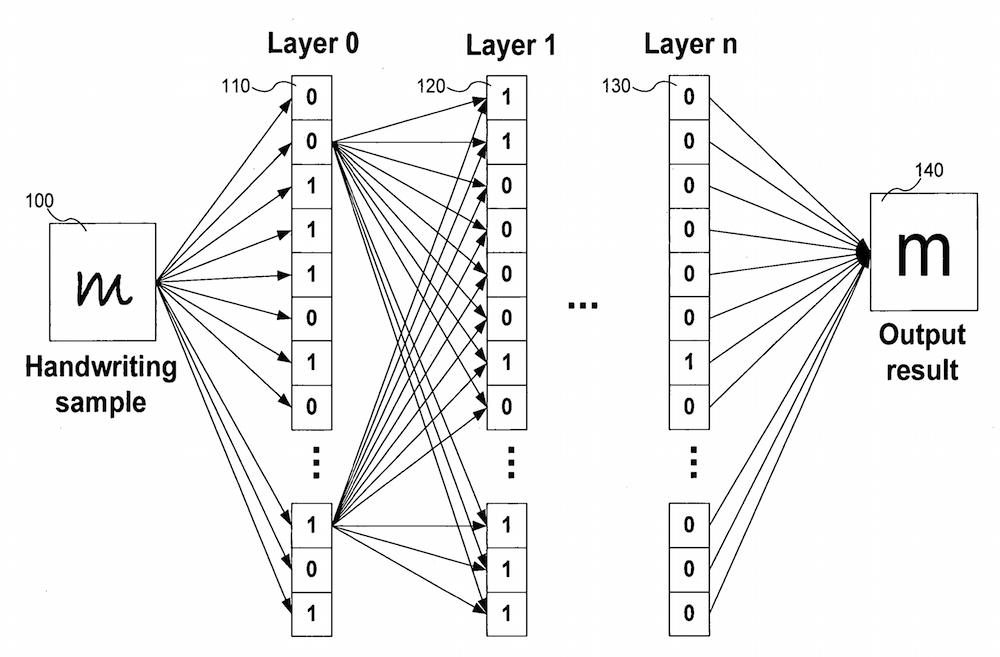
\includegraphics[width=\textwidth]{graph.png}
\caption{Resolution of pictures should be at least 300 dpi.\label{fig1:fig}}
\end{figure}%

Refer to figures and tables like Fig.~\ref{fig1:fig} and Table~\ref{tab:perf}.

\section*{[CONCLUDING REMARKS]}
We provide an example for using the \LaTeX\ Template of the Journal of Information Science and Engineering. Any questions or bugs can be sent to the editor \cite{wang2010taintscope,chen2018angora}.
\fi

\section*{ACKNOWLEDGMENT}
This is the Acknowledgment section. Note that it is unnumbered.


\bibliographystyle{JISEbib}
\bibliography{ref}
%\bibliography{references}

\begin{IEEEbiography}[{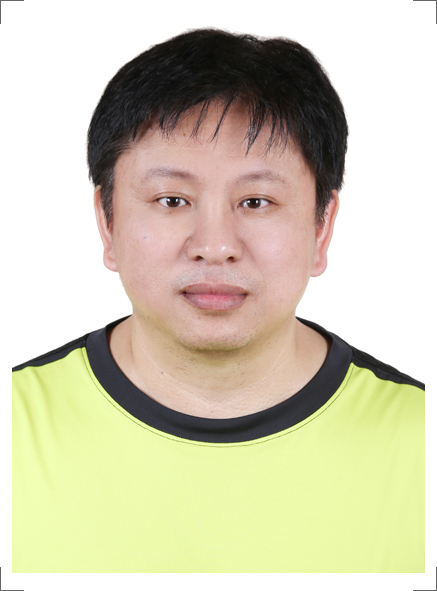
\includegraphics[width=3cm,height=4cm]{njhuang.jpg}}]{Nan-Jung Huang}
received his B.S. (1988) degree in Computer Science and Information Engineering from National Chiao Tung University in Taiwan, and M.S. degree (1994) in the Department of Computer Science and Engineering from Mississippi State University, USA. He is currently a Ph.D. candidate in the Department of Computer Science at National Yang Ming Chiao Tung University. Mr. Huang's research focuses on software testing with an emphasis on taint analysis and multi-target directed fuzzing.
\end{IEEEbiography}

\begin{IEEEbiography}[{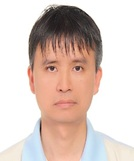
\includegraphics[width=3cm,height=4cm]{skhuang.jpg}}]{Shih-Kun Huang}
received his B.S. (1989), M.S. (1991), and Ph.D. (1996) degrees in Computer Science and Information Engineering from National Chiao Tung University. From 1996 to 2004, he served as an Assistant Research Fellow at the Institute of Information Science, Academia Sinica. He is currently a professor at the Information Technology Service Center and holds a joint appointment with the Department of Computer Science at National Chiao Tung University. Dr. Huang's research focuses on the integration of software engineering and programming languages, with an emphasis on cybersecurity and software vulnerability analysis.
\end{IEEEbiography}

\begin{IEEEbiography}[{
\includegraphics[width=3cm,height=4cm]{AlaRduTP_s.png}}]{Ying-TA Chen}
received his M.S. (2025) degree in Department of Computer Science from National Yang Ming Chiao Tung University in Taiwan. Mr. Chen's research focuses on the integration of software engineering and programming languages, with an emphasis on cybersecurity and software vulnerability analysis.
\end{IEEEbiography}

\end{document}
